%特別研究論文
\documentstyle[11pt,a4j,makeidx,ascmac,epsbox,ronbun,hyoushi,fig_tab,theorem,list,cprog,graphicx,comment]{jreport}
	\newcommand{\ve}[1]{\mbox{\boldmath{$#1$}}}
	\def\rubyfont{\tiny}
	\makeatletter
	\def\ruby#1#2{\leavevmode\vbox{%
	\baselineskip\z@skip\lineskip.25ex
	\ialign{##\crcr\rubyfont\hfill#2\hfill\crcr
	\hfill#1\hfill\crcr}}}
	\textwidth 6.5in
	\textheight 9.5in
	\oddsidemargin .2in
	\topmargin -.5in
	\parindent 1zw
	\makeindex
	
\begin{document}

\large
	%\maketitle
	%#!jlatex main.tex
{\large
\title{\Large{\underline{特別研究}}\\
\vspace{0.5cm}

}}
\author{}
\maketitle
	\pagenumbering{roman}
	\tableofcontents\newpage
	\listoffigures\newpage
	\listoftables\newpage
	\pagebreak
	\pagenumbering{arabic}

\chapter{緒言}
\section{研究背景}

\section{先行研究例}

\section{研究目的}

\section{論文構成}
本論文の構成は以下の通りである.
{\bf 第2章}で述べ,{\bf 第3章}で計測アルゴリズムと実験手法に関して示す.
{\bf 第4章}では結果を示し、に関して考察する.
最後に{\bf 第5章}で本論文の成果をまとめる.

\chapter{動作モデル・実験器具製作}
\section{動作モデル}
\subsection{ストレッチセンサ}
ストレッチセンサはFig.\ref{fig:ストレッチセンサ全体図},Fig.\ref{fig:ストレッチセンサ断面図}において示す通り,
柔軟で弾性変形する伸縮性シリコン(絶縁層)と導電性布電極(導電層)の重ね合わせによって構成されている.
これは,誘電体をシリコン,極板を導電性布としたコンデンサとなっている.

\begin{figure}[h]
    \begin{center}
        \label{fig:ストレッチセンサ全体図}
        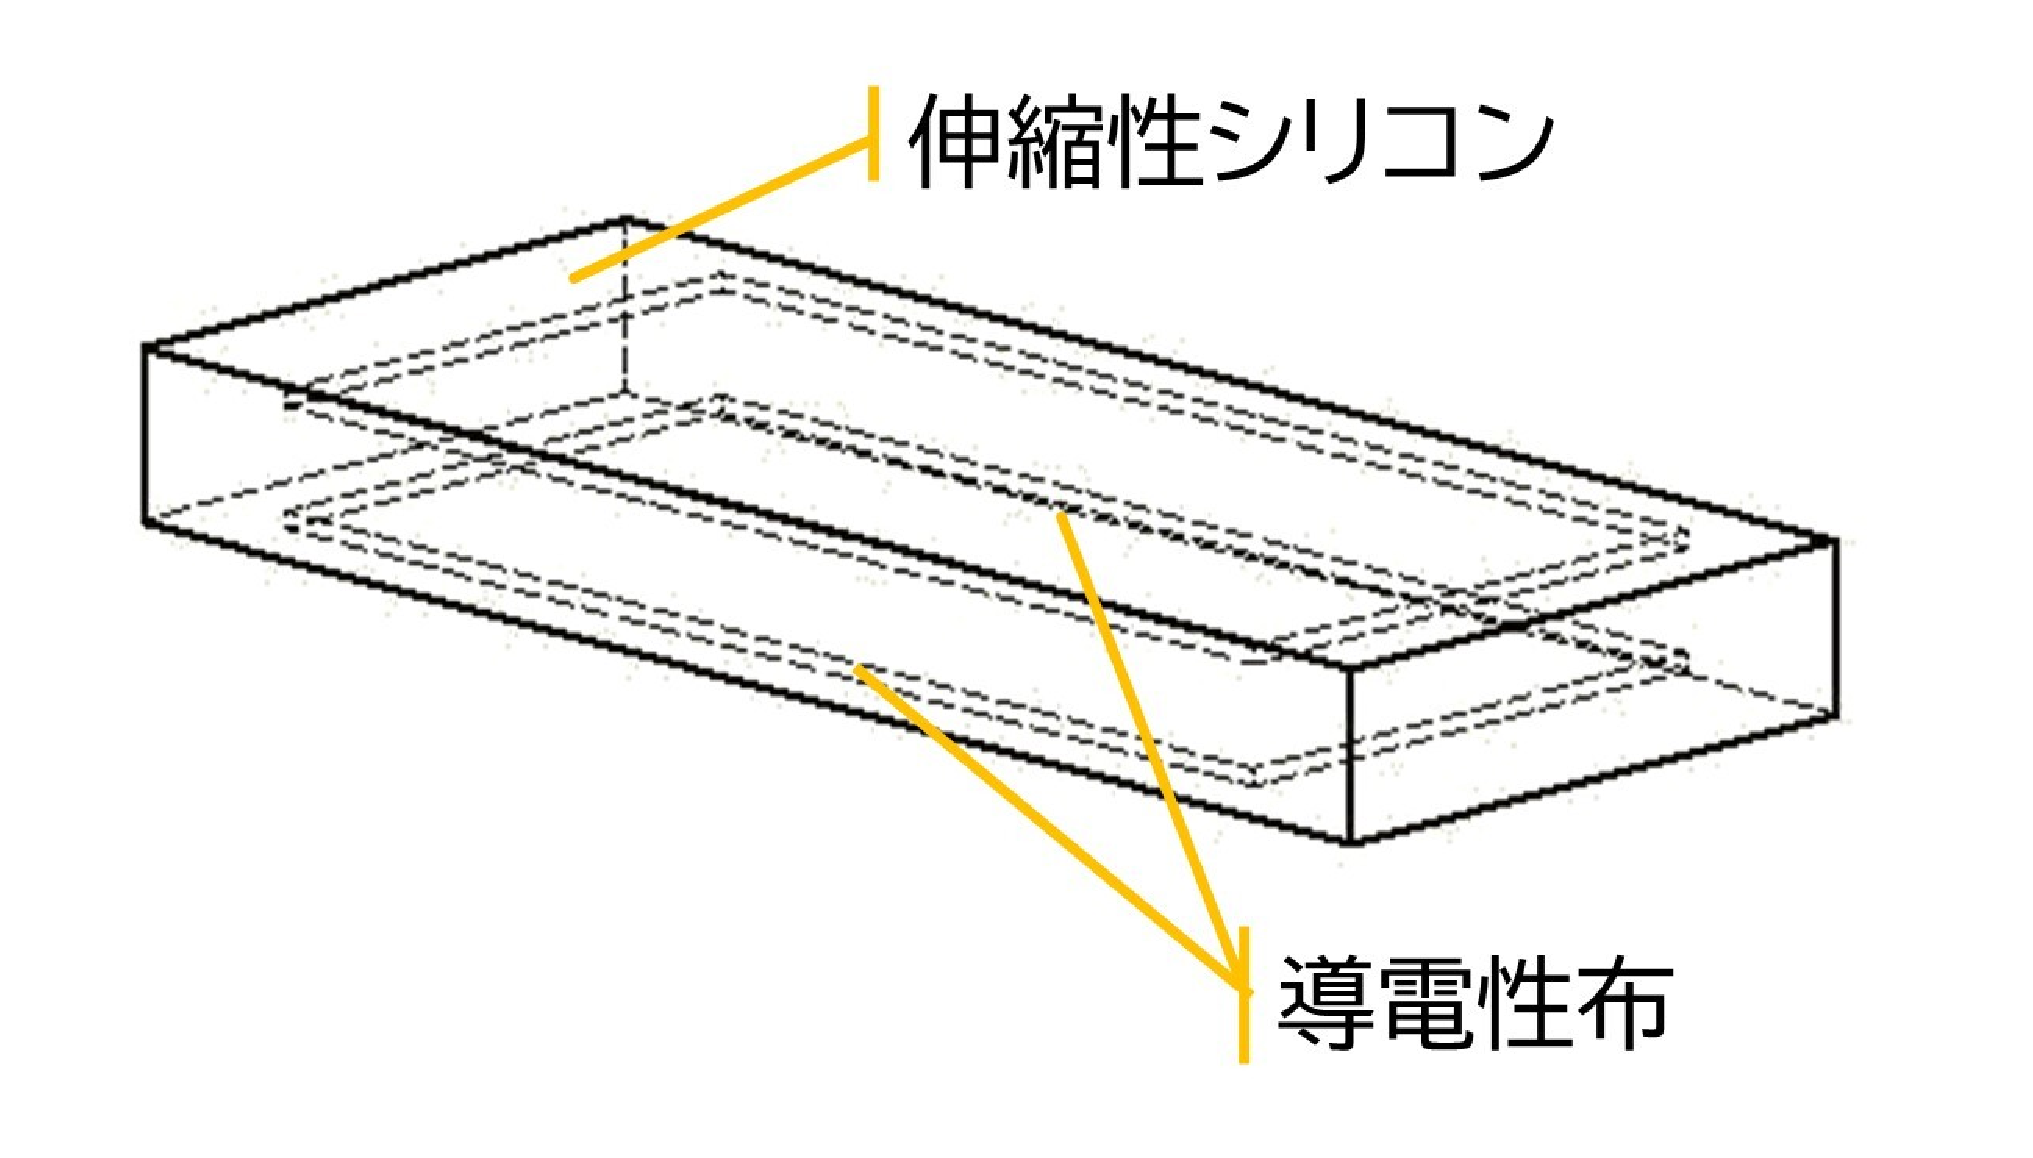
\includegraphics[width=0.4\columnwidth,clip]{./2_measurement/slide1.eps}
        \caption{ストレッチセンサ全体図}     
        \label{fig:ストレッチセンサ断面図}
        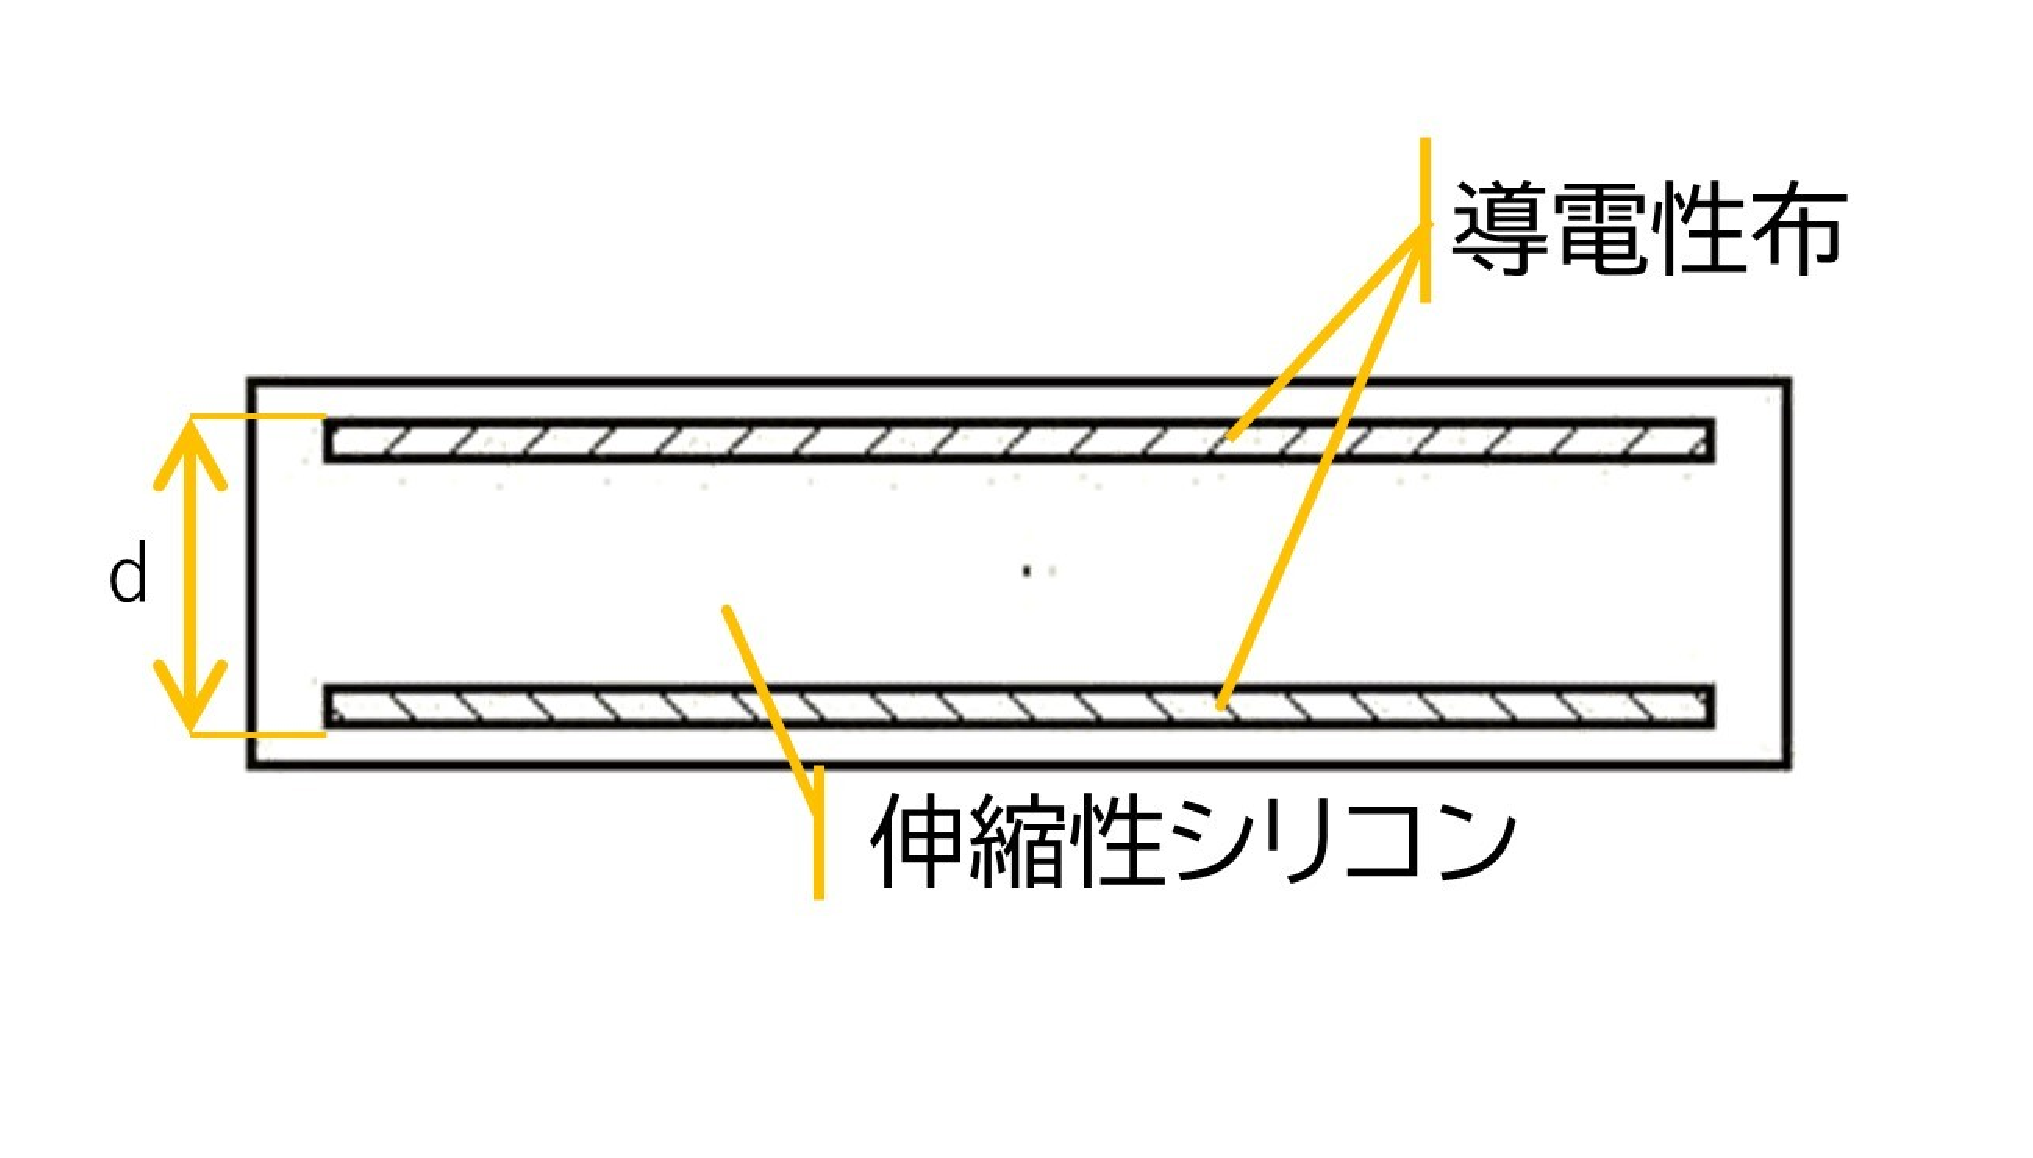
\includegraphics[width=0.4\columnwidth,clip]{./2_measurement/slide2.eps}
        \caption{ストレッチセンサ断面図}
    \end{center}
\end{figure}

ここでストレッチセンサ中の導電性布の長さ$l$,幅$w$,シリコンの厚さを$d$,シリコンの誘電率を$\epsilon{}_s$とすると,
\begin{eqnarray}
    C=\epsilon{}_s\frac{lw}{d}
    \label{eq:cap}
\end{eqnarray}
といった式でその静電容量$C$が求められる.この式からもわかる通り,シリコンの誘電率を$\epsilon{}_s$を
一定と考えると,静電容量のパラメータとして,導電性布の長さ$l$,幅$w$,シリコンの厚さ$d$が
挙げられる.ストレッチセンサに引張方向に力を加えると,これらが変化する.今回は,ストレッチセンサに
対する引張方向の長さの変化を,ストレッチセンサの静電容量の変化として計測するシステムの開発を行った.

\subsection{ストレッチセンサ計測回路}\label{sec:RC回路}
%TODO:ストレッチ計測回路に関しての記述を行う
先述の通り,ストレッチセンサは静電容量の変化で伸縮状況を示す.故に今回は静電容量の変化を計測することが
できる回路の製作を行った.静電容量の計測を行う方法として,LRCメータやインピーダンスアナライザを
用いる方法が挙げられる.これらの計測機器を用いると静電容量の変化を高精度に計測することができる.
しかし,1ch当たりの計測機器の単価が非常に高く,また既存のフィードバック系に組み込みにくいといった状況が
あった.そこで,今回はより安価で手軽な方法である,RC回路を用いた方法をとった.

下記のFig.\ref{fig:RC}に示したRC回路を用い,Vinに入力を与えるとVoutで信号が立ち上がるまでに
時間遅れが発生する.これは,抵抗値$R$,静電容量$C$とすると,時定数$\delta t$は,
\begin{eqnarray}
    \delta t = RC
\end{eqnarray}
といった式であらわされる.なお,この遅れ系の現象を計測すると,Fig.\ref{fig:oscilloscope}の様になる.

これらの計測に関して,1つのマイコンを用いて複数のストレッチセンサの計測を行うと計測周期が低下し,
計測精度の低下が懸念された.これを踏まえ,1つのマイコンで計測を行うストレッチセンサの数を1個とした.
一方で今回,足首を中心とした筋の伸縮の計測を行うため3チャンネル分の計測を行う必要がある.
故に,マイコン3枚分の計測システムを用意した.これらを計測用PCでSerial通信を用いてデータの取得を行った.
\begin{figure}[h]
    \begin{center}
        %TODO:Voutの向きを出力にする
        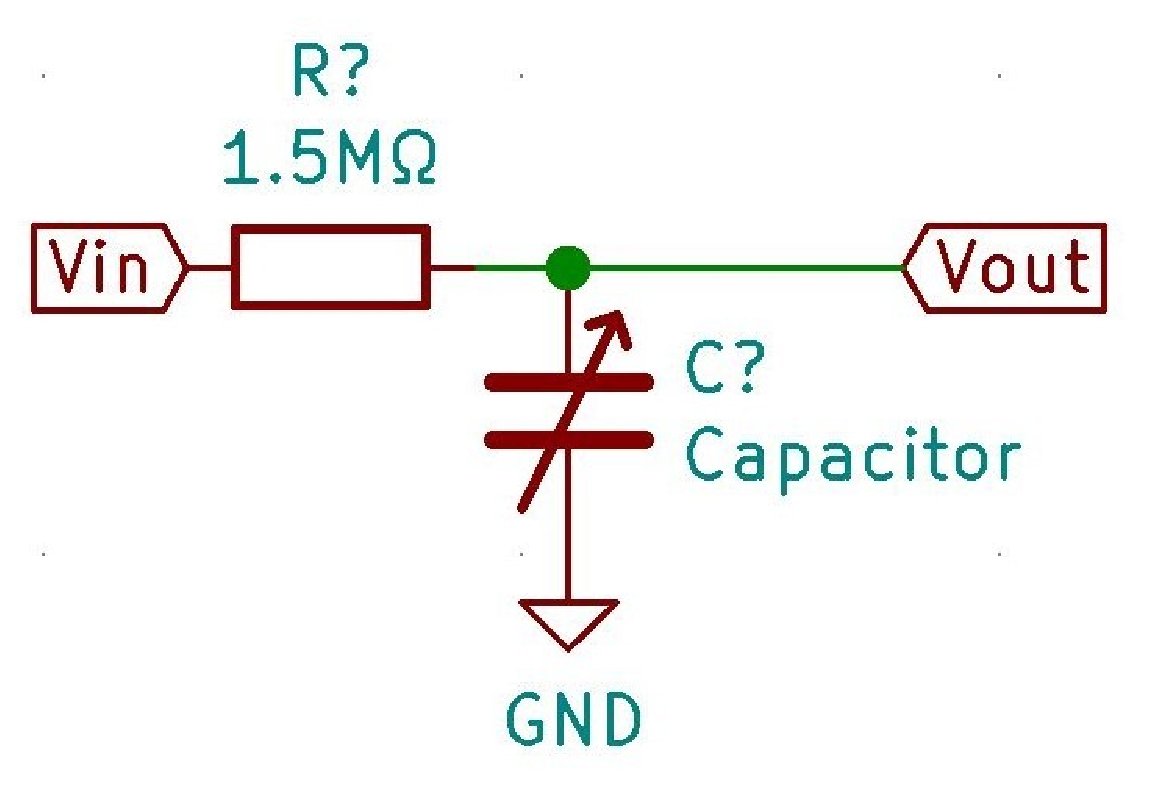
\includegraphics[width=0.4\columnwidth,clip]{./2_measurement/RC.eps}
        \caption{RC回路}
        \label{fig:RC}
        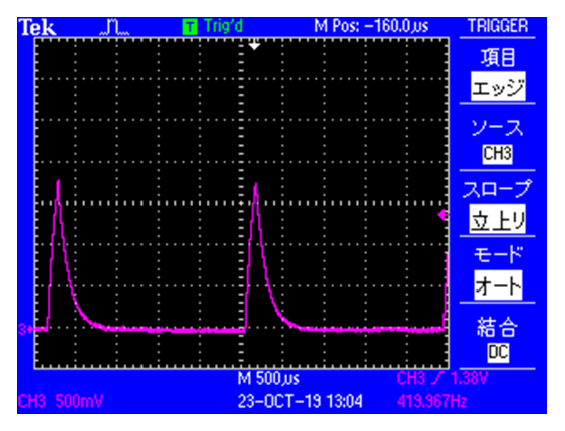
\includegraphics[width=0.4\columnwidth,clip]{./2_measurement/oscilloscope.eps}
        \caption{出力状態図}
        \label{fig:oscilloscope}
    \end{center}
\end{figure}

\newpage

\subsection{足関節における筋肉}
Fig.\ref{fig:legMuscle}において,脚部における筋肉状況を示す.これらの脚部筋肉のうち足関節の動作に
寄与している物はヒラメ筋,長腓骨筋,前脛骨筋,長母趾伸筋,長趾伸筋といったものが挙げられる.

従来のペダリングロボット,2足歩行ロボットの足関節部分では前脛骨筋,ヒラメ筋のみに注目し
それらの筋肉の再現を,空気圧人工筋を用いて行った.
今回製作する足関節ロボットでは実際の人間の動作の再現を行うため,従来のピッチ方向のみの動作を
想定した設計では目的を満たすことができない.そこで,従来注目していた,前脛骨筋,ヒラメ筋に
加えて,長腓骨筋も注目するようにした.また,従来のロボットでは足関節部分はピンジョイントを用いて,
動作方向の制限を行っていたが,今回はボールジョイントを用い,動作方向の制限をなくし,ロール・ピッチ・ヨー各方向に
自由度を持たせることができた.
\begin{figure}[h]
    \begin{center}
     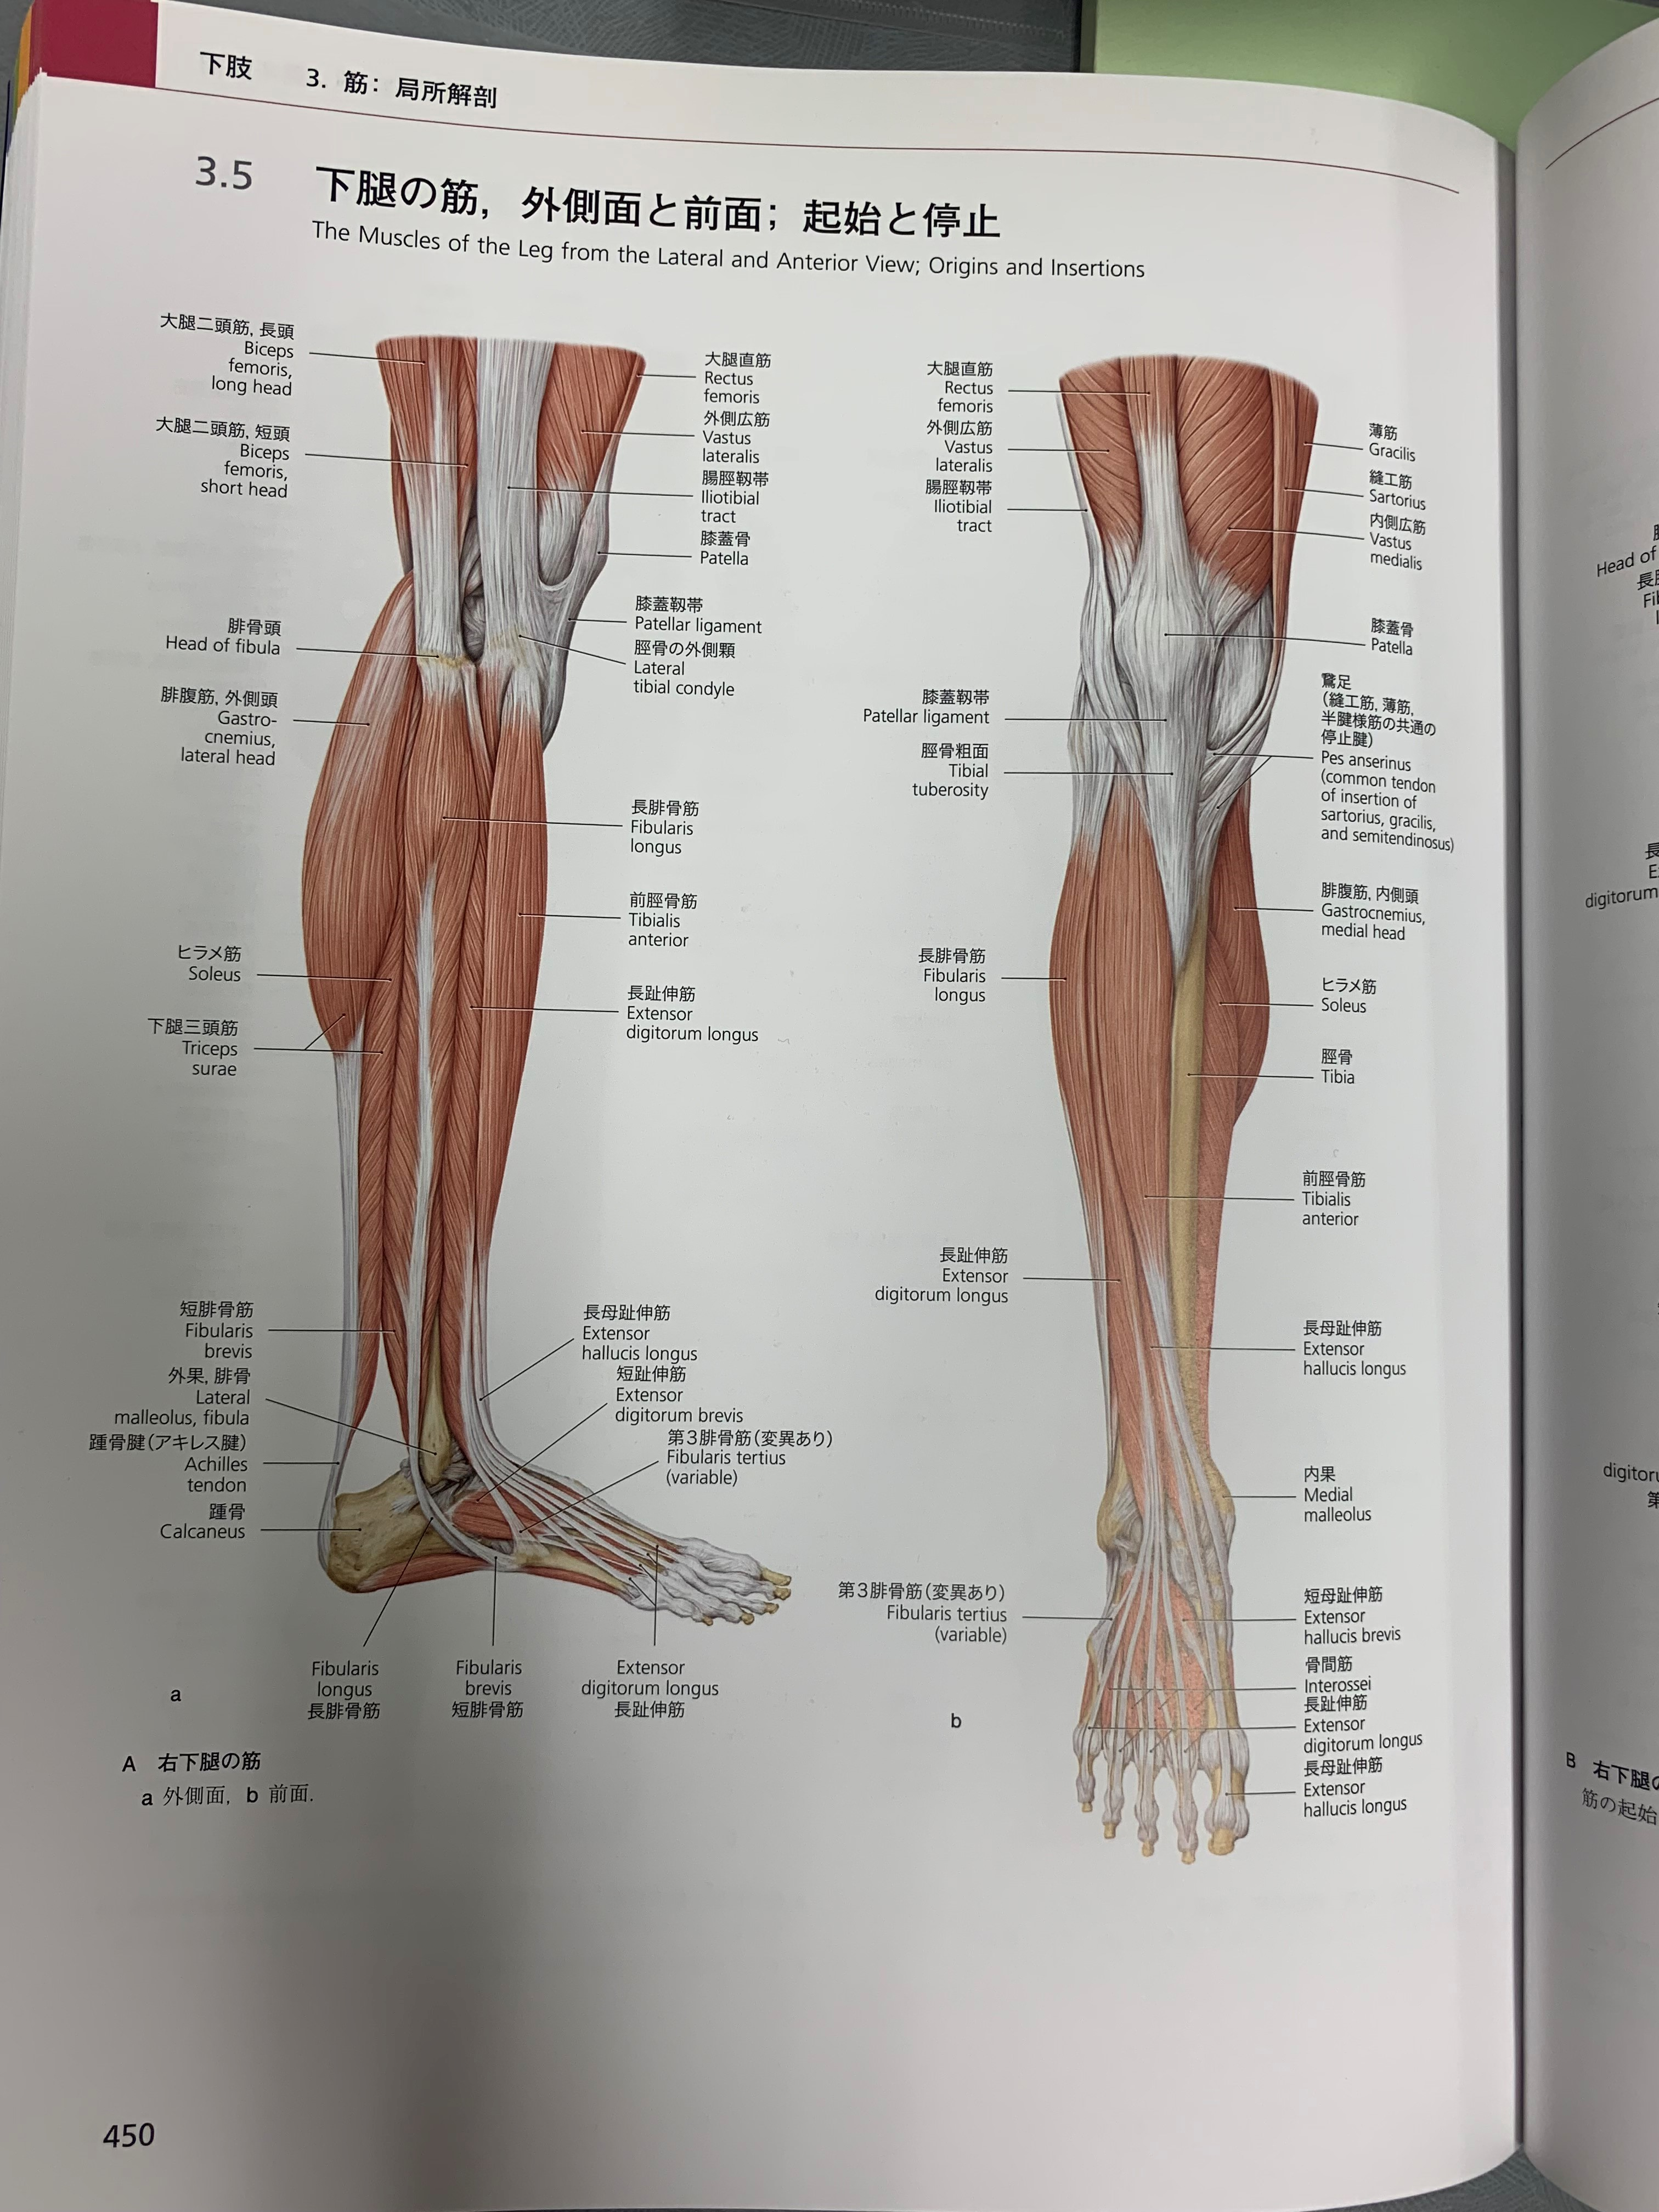
\includegraphics[width=0.5\columnwidth,clip]{./2_measurement/legMuscle.eps}
     \caption{脚部における筋肉状況}
     \label{fig:legMuscle}
    \end{center}
\end{figure}

\newpage

\section{実験器具の製作}
今回,ストレッチセンサとその計測回路,また足関節ロボットの製作を行った.以下にそれらの製作過程の記述を行う.
\subsection{ストレッチセンサ}
まず,Fig.\ref{fig:Inventor}の様に3DCADであるInventorを用いて,ストレッチセンサとして使用するシリコン材を流し込むための型の設計を行う.
設計を行ったCADデータをもとに,3Dプリンタ(Afinia H800)を用いてABS樹脂で型の出力を行う.出力を行った型はFig.\ref{fig:3Dprinter}にて示すものである.

\begin{figure}[h]
    \begin{center}
        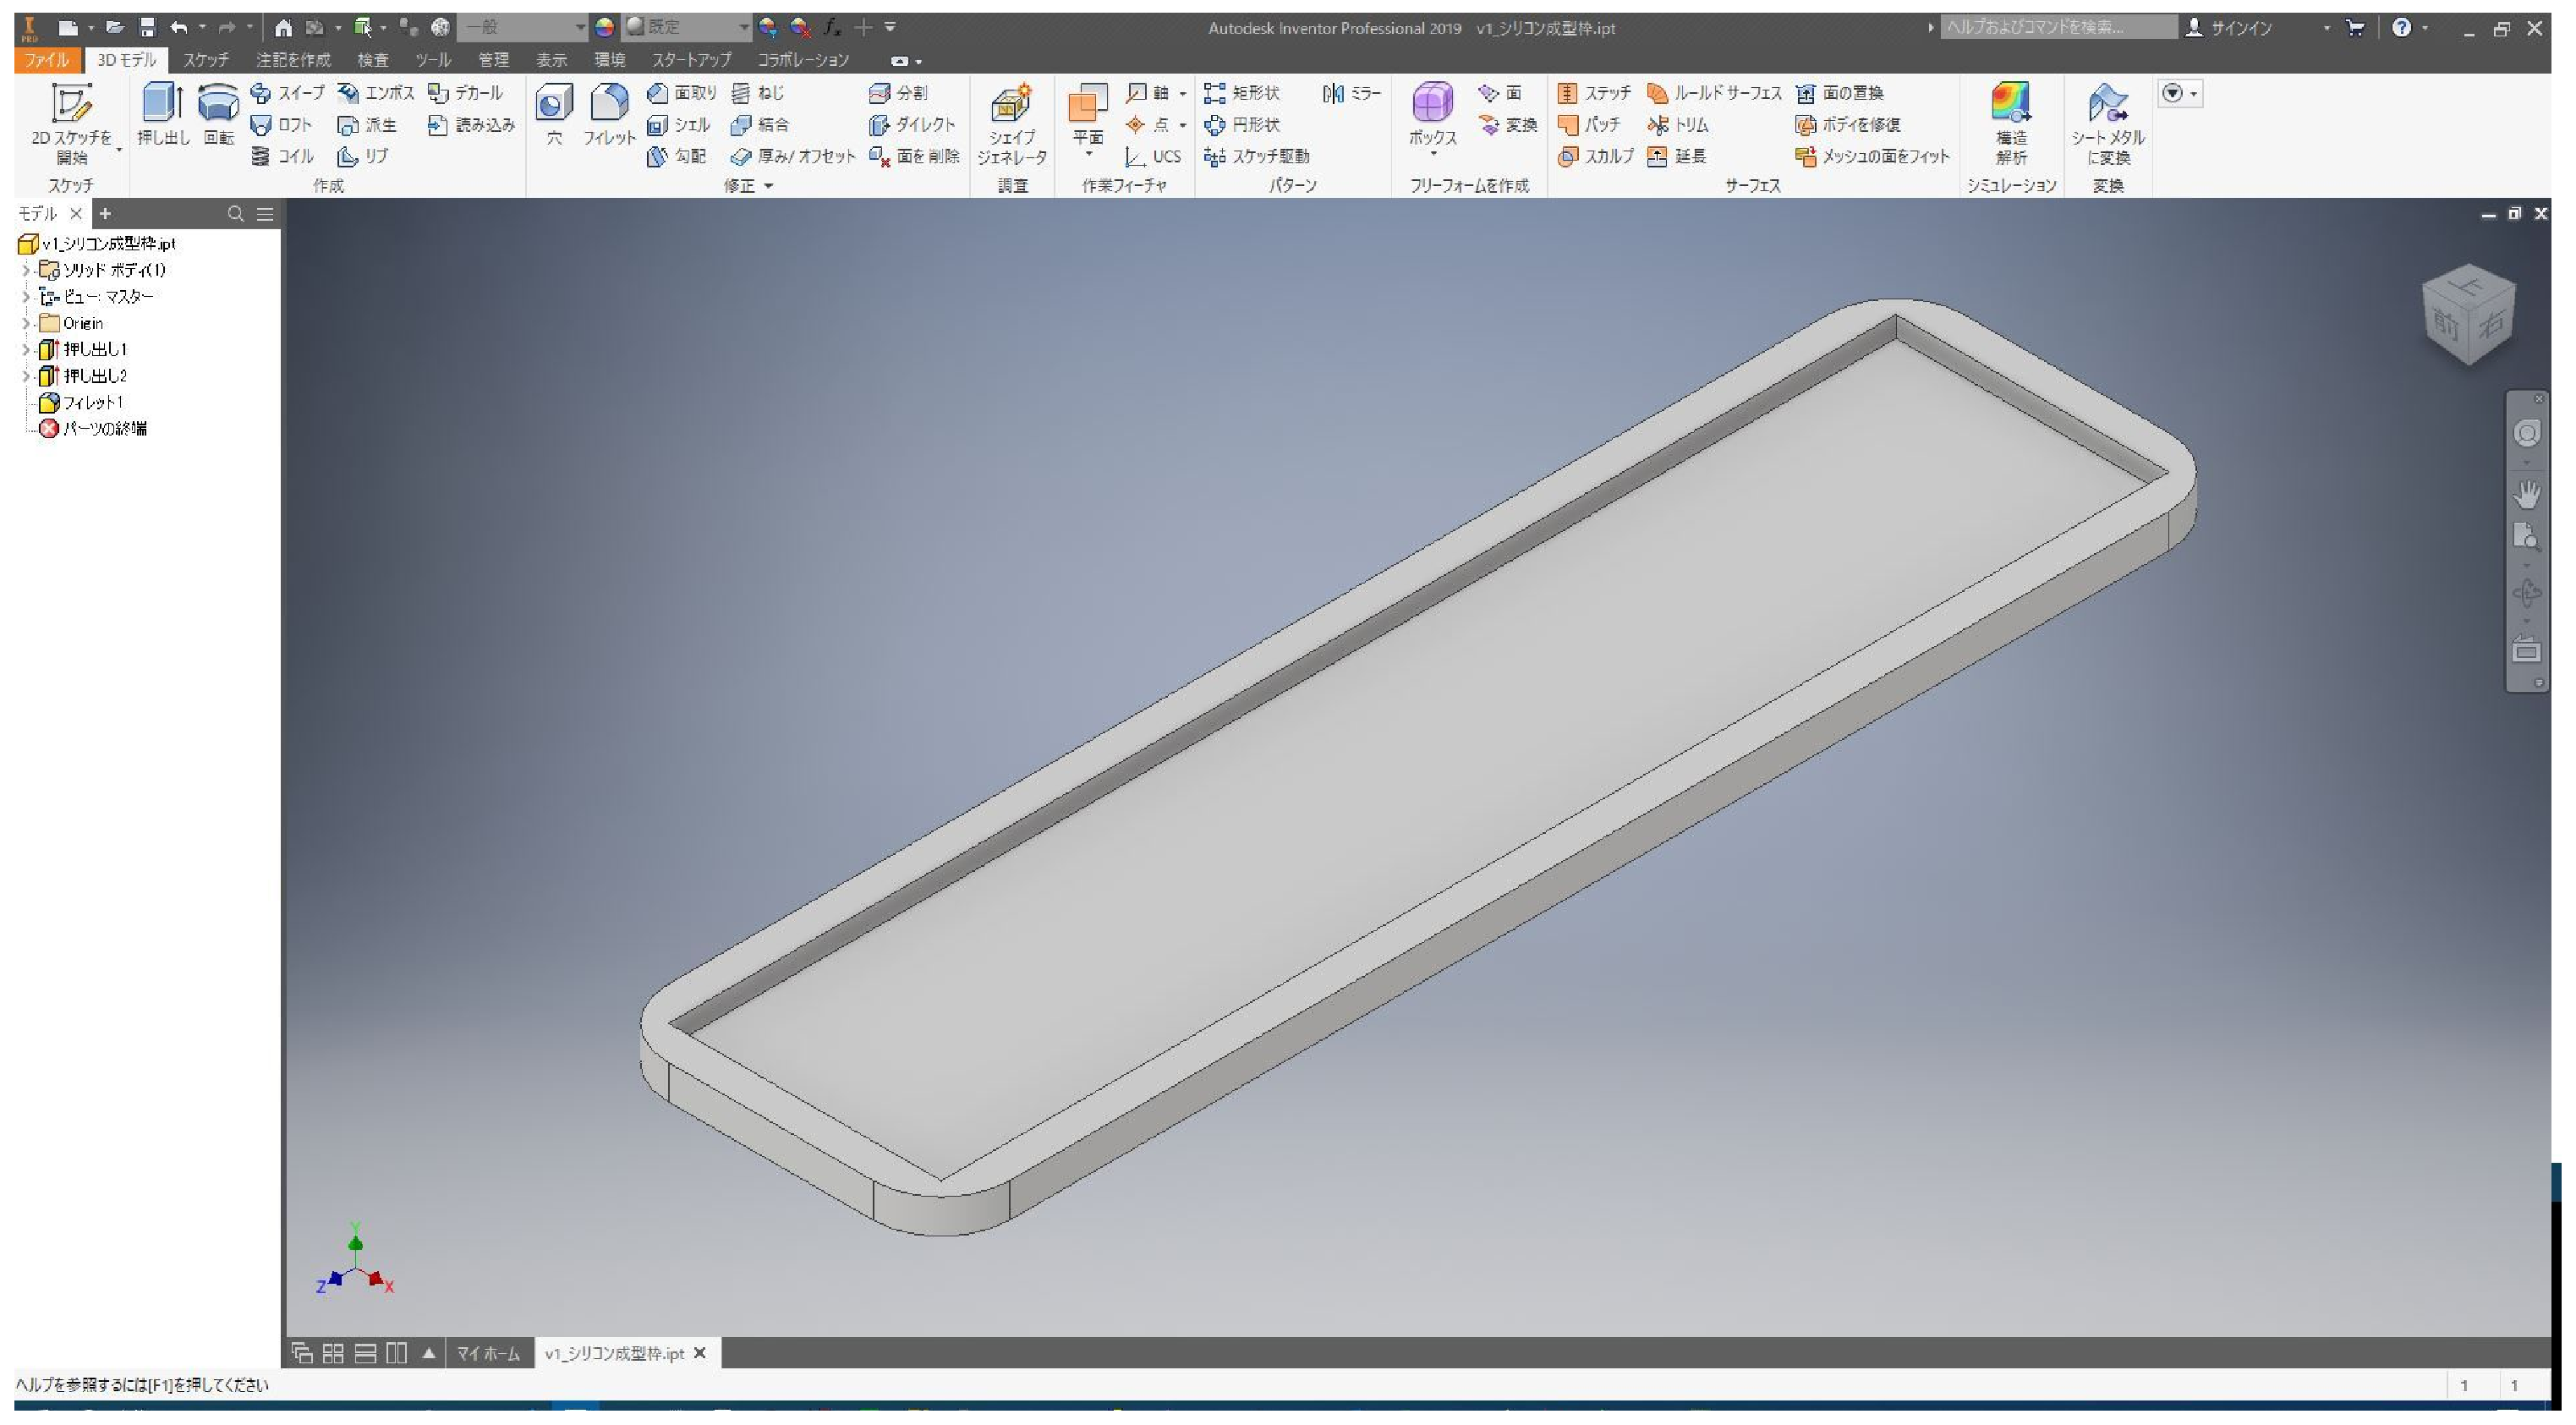
\includegraphics[width=0.6\columnwidth,clip]{./2_measurement/inventor.eps}
        \caption{Inventorを用いて設計した状況}
        \label{fig:Inventor}
    \end{center}
\end{figure}
\begin{figure}[h]
    \begin{center}
        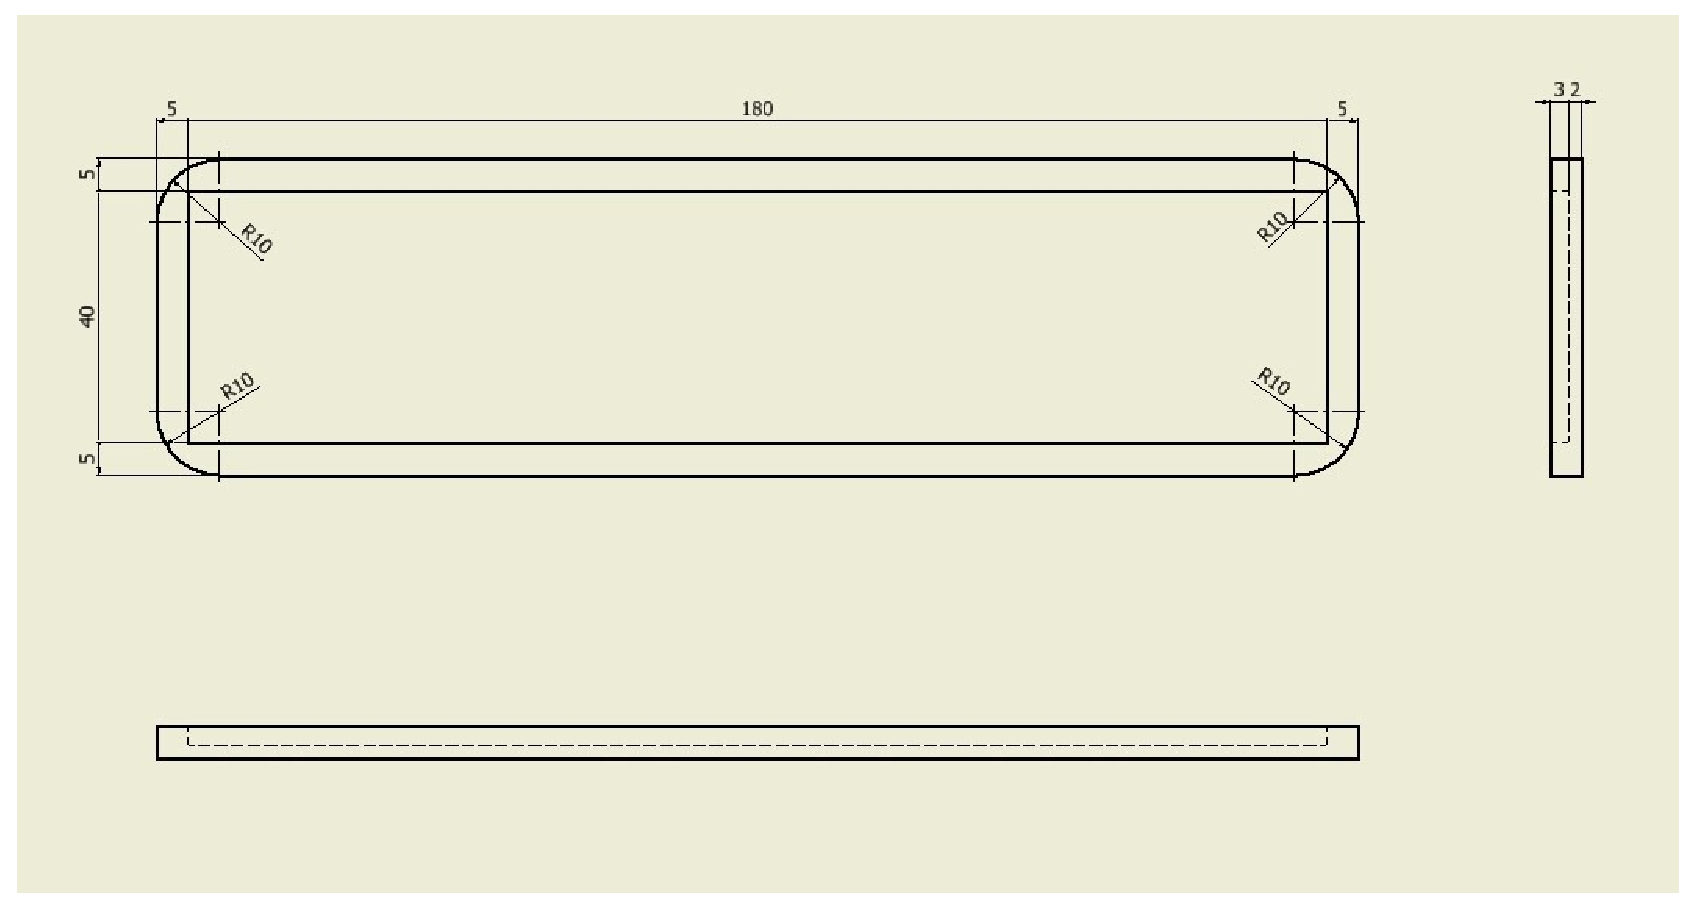
\includegraphics[width=0.6\columnwidth,clip]{./2_measurement/drowing.eps}
        \caption{設計した型(図面)}
        \label{fig:3Dprinter}
    \end{center}
\end{figure}
\begin{figure}[h]
    \begin{center}
        
\includegraphics[width=0.6\columnwidth,clip]{./2_measurement/3dprint.eps}
        \caption{3Dプリンターで出力された型}
        \label{fig:3Dprinter}
    \end{center}
\end{figure}

\newpage
続いて,3Dプリンターにて出力した型に合わせて,導電性布をはさみで切る.導電性布に錫めっき線を縫い通し,型の上に置く.
この際,錫めっき線が型の外に出てくるようにする.その上から硬化剤を混ぜたシリコン20g程を流し込み固まるまで数時間放置する.
なお,使用したシリコンと硬化剤は,Fig.\ref{fig:silicon}にて示すものである.シリコンが固まったら2枚目の導電性布に1枚目と同様に
錫めっき線を通し硬化したシリコンの上に置く.その上から硬化剤を混ぜたシリコン5gを薄く塗り固まるまで放置する.最後のシリコンが
硬化したら型から取り外し,錫めっき線にはんだを用いて銅線を接続し,コネクタを圧着して完成となる.

\begin{figure}[h]
    \begin{center}
        
\includegraphics[width=0.6\columnwidth,clip]{./2_measurement/silicon.eps}
        \caption{製作に使用したシリコンと硬化剤}
        \label{fig:silicon}
    \end{center}
\end{figure}

\newpage
\subsection{ストレッチセンサ計測回路}

先述の通り,ストレッチセンサの静電容量計測にはRC回路を用いた.また,その計測用マイコンとして,NucleoF303K8を用いた.
その回路設計に関して,以下に記述する.

まず,KiCADを用いて回路図の設計を行った.その結果,Fig.\ref{fig:circuitPic}に示すようになった.
続いて,KiCADを用いてPCB基板の設計を行った.設計結果は,Fig.\ref{fig:PCB}に示す様になった.
なお,Fig.\ref{fig:circuitPic}に示した回路以外のものも今後の研究のため搭載されているが今回の研究に関わるものだけを抜粋して示した.
そして,その設計データを元にPCB基板の外注を行った.そして,基板にパーツをはんだ付けし完成となった.
完成したものは,Fig.\ref{fig:circuit}に示したものである.

\begin{figure}[h]
    \begin{center}
        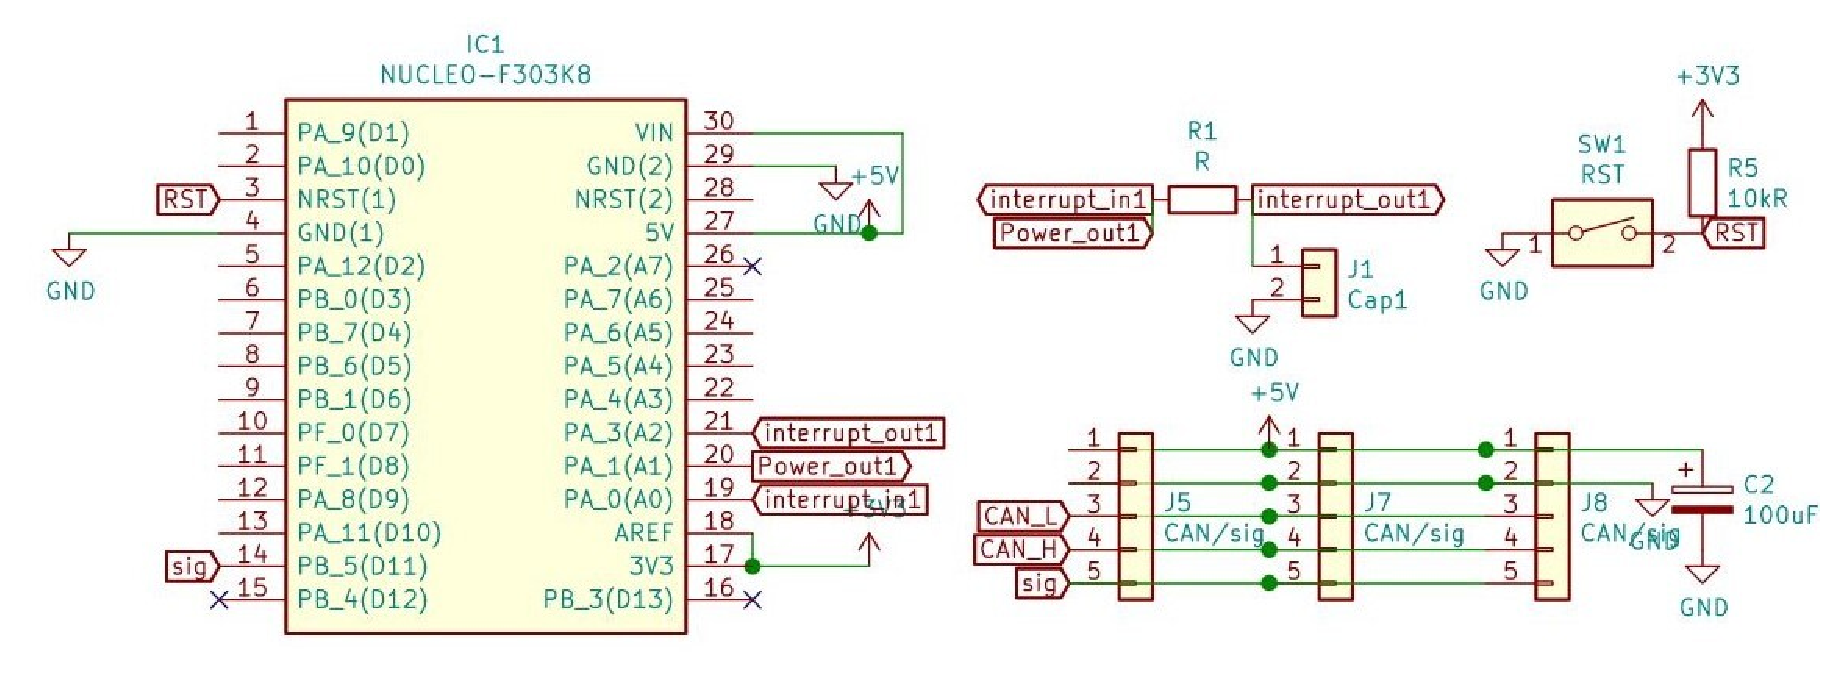
\includegraphics[width=0.7\columnwidth,clip]{2_measurement/circuitPicture.eps}
        \caption{計測回路図}
        \label{fig:circuitPic}
    \end{center}
\end{figure}
\begin{figure}[h]
    \begin{center}
        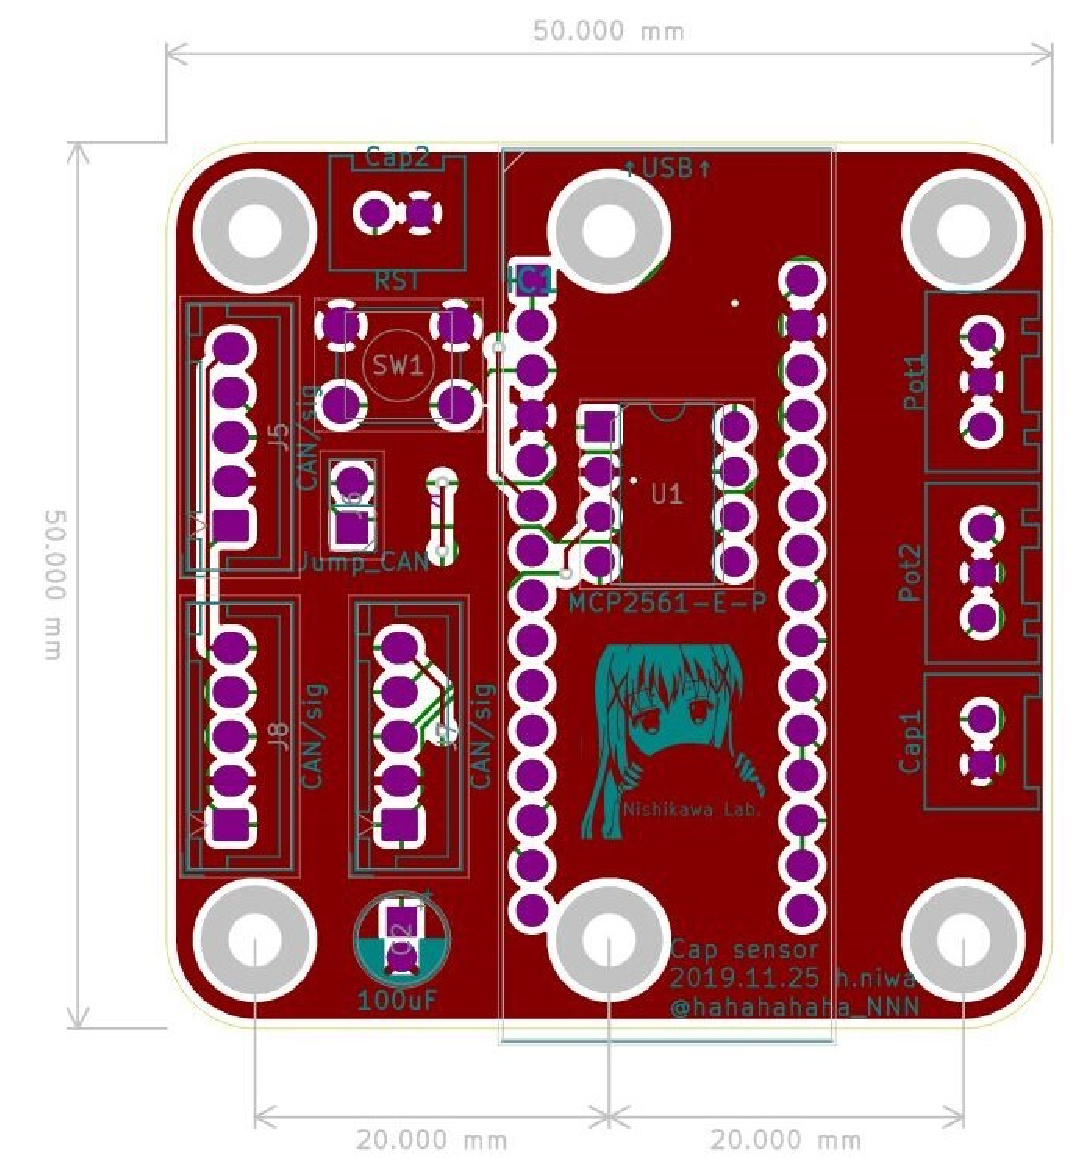
\includegraphics[width=0.4\columnwidth,clip]{2_measurement/PCB.eps}
        \caption{PCB基板設計図}
        \label{fig:PCB}
    \end{center}
\end{figure}
\begin{figure}[h]
    \begin{center}
     
\includegraphics[width=0.6\columnwidth,clip]{./2_measurement/circuit.eps}
     \caption{計測に用いた基板}
     \label{fig:circuit}
    \end{center}
\end{figure}

\subsection{足関節ロボット}
%TODO:使用した人体模型の種類の記述を行う.

今回,足関節ロボットの骨格としてFig.\ref{fig:bodyBone}の人体模型を用いた.本模型から必要となる,膝より下の部分を取り外した.
取り外した結果,Fig.\ref{fig:legBone}の様になった.
\begin{figure}[h]
    \begin{center}
     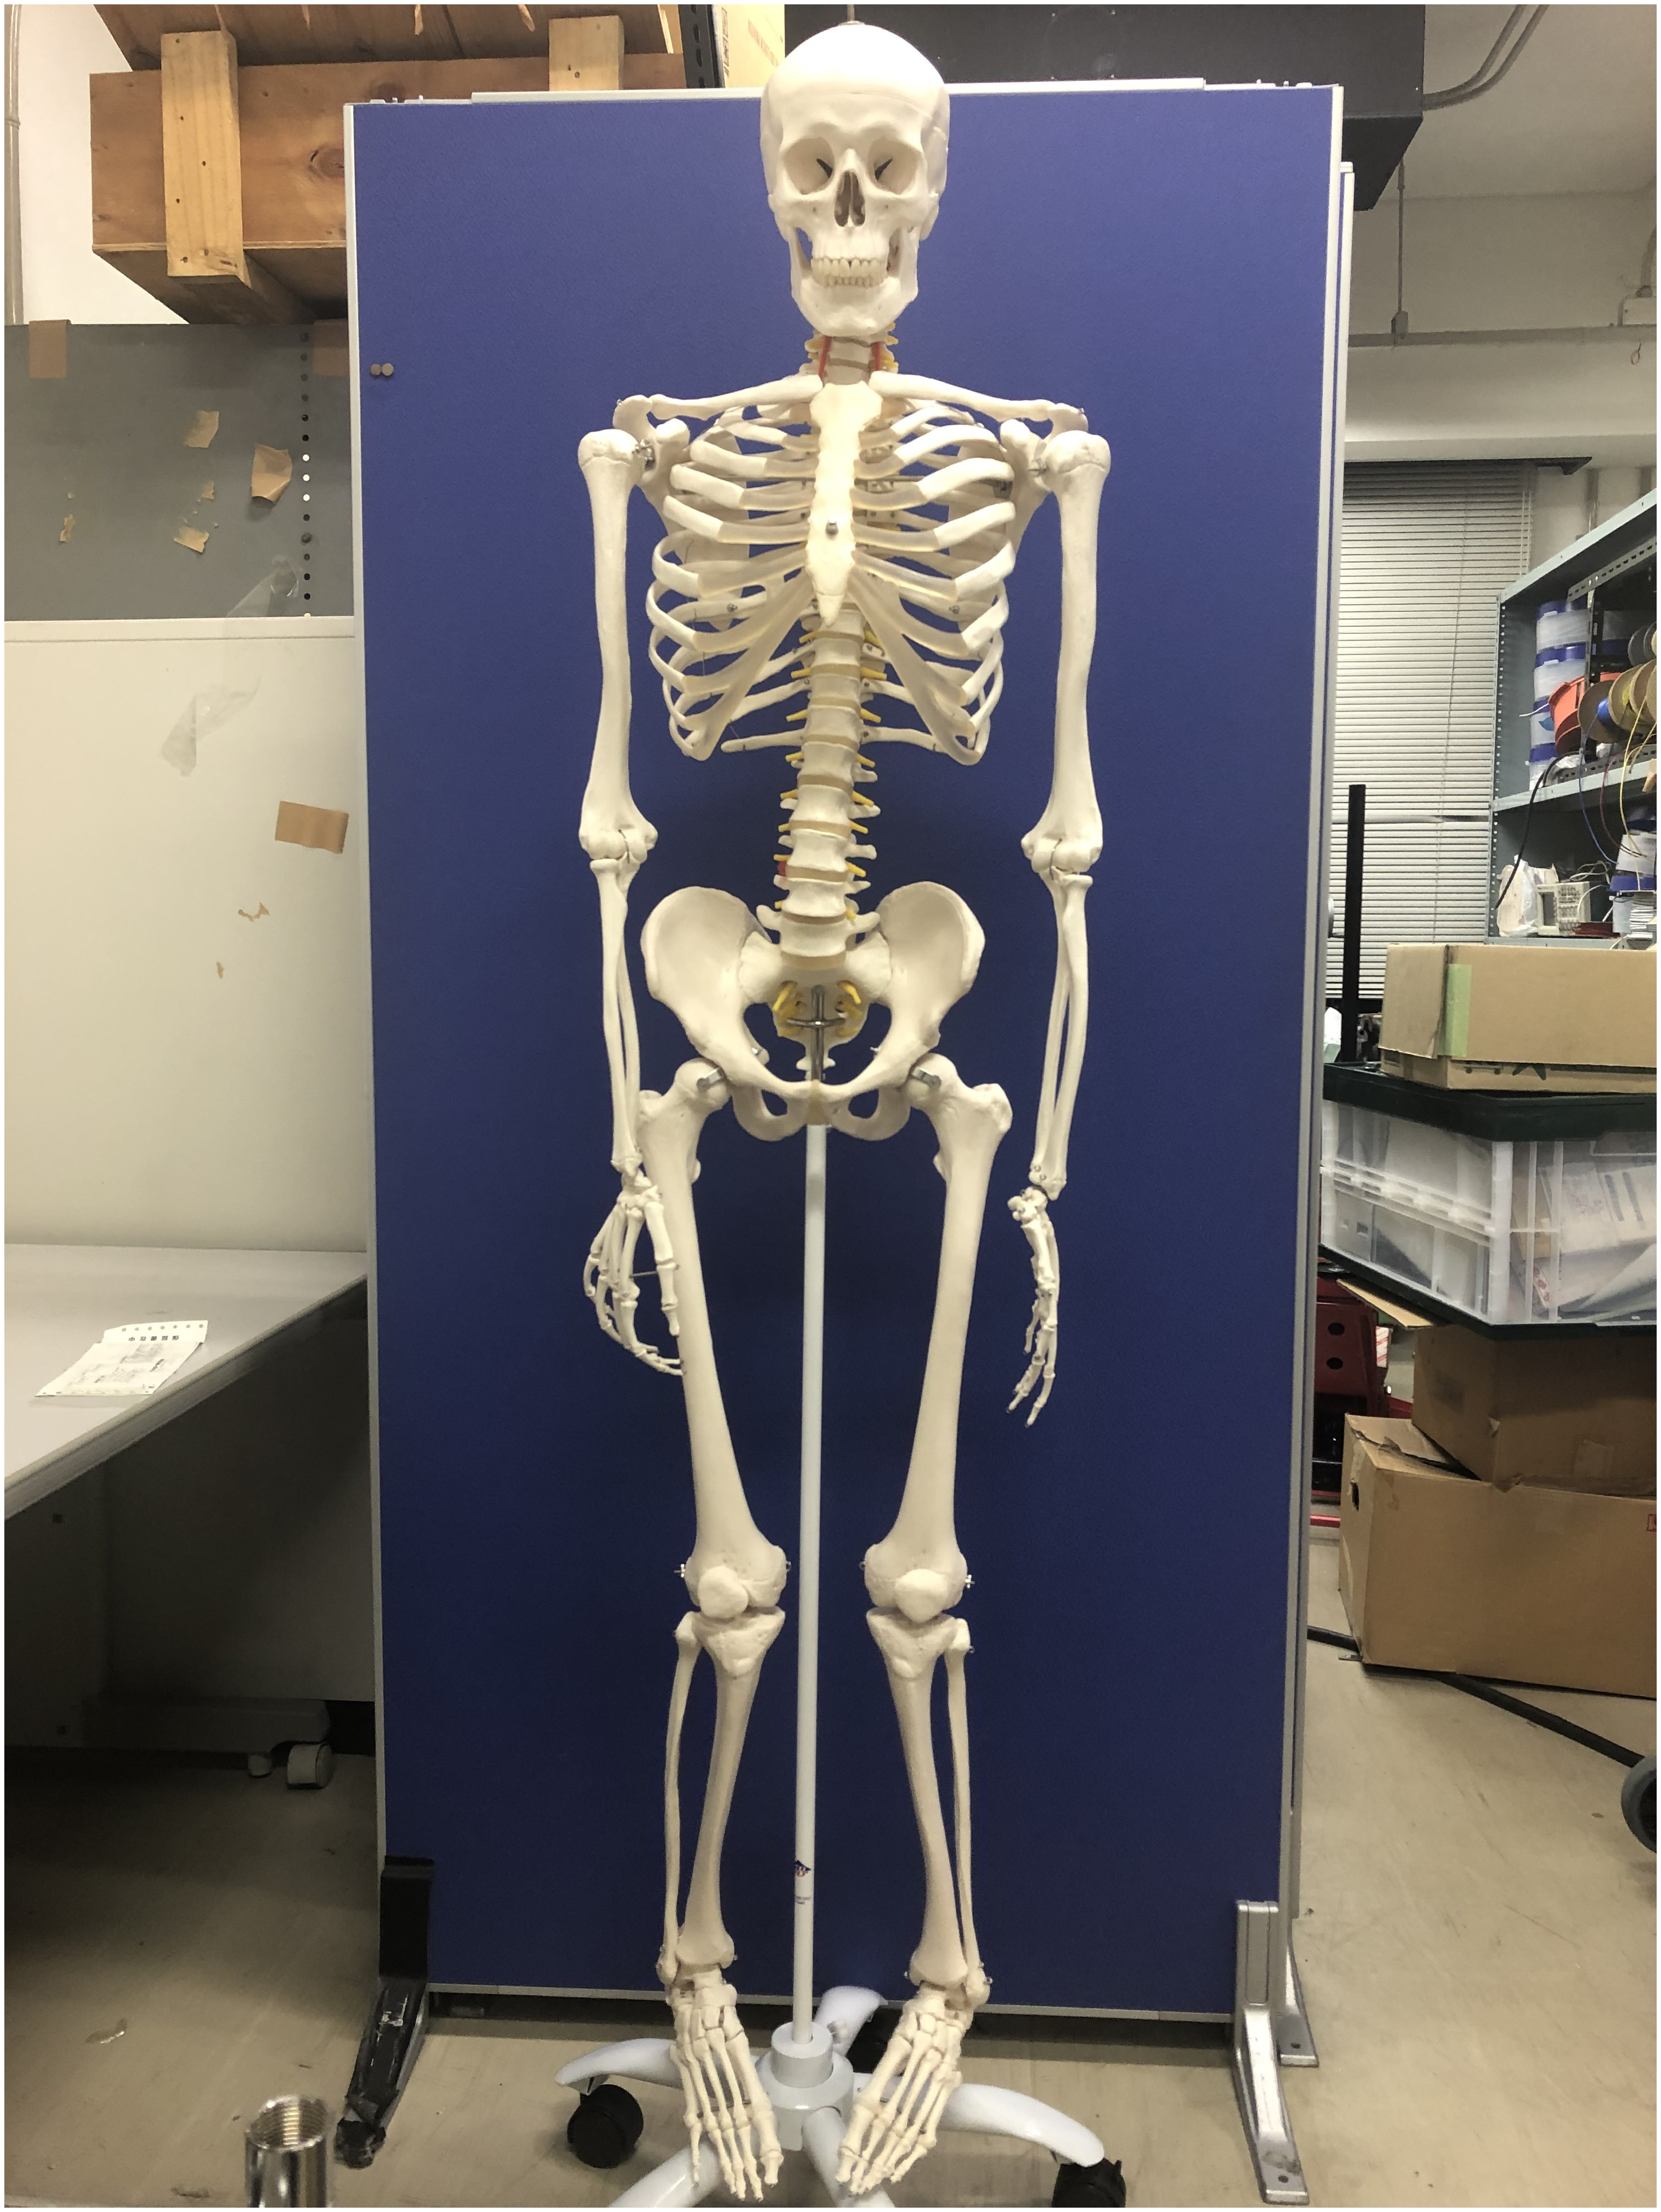
\includegraphics[width=0.4\columnwidth,clip]{./2_measurement/bodyBone.eps}
     \caption{人体模型骨格(全身)}
     \label{fig:bodyBone}
    \end{center}
\end{figure}
\begin{figure}[h]
    \begin{center}
     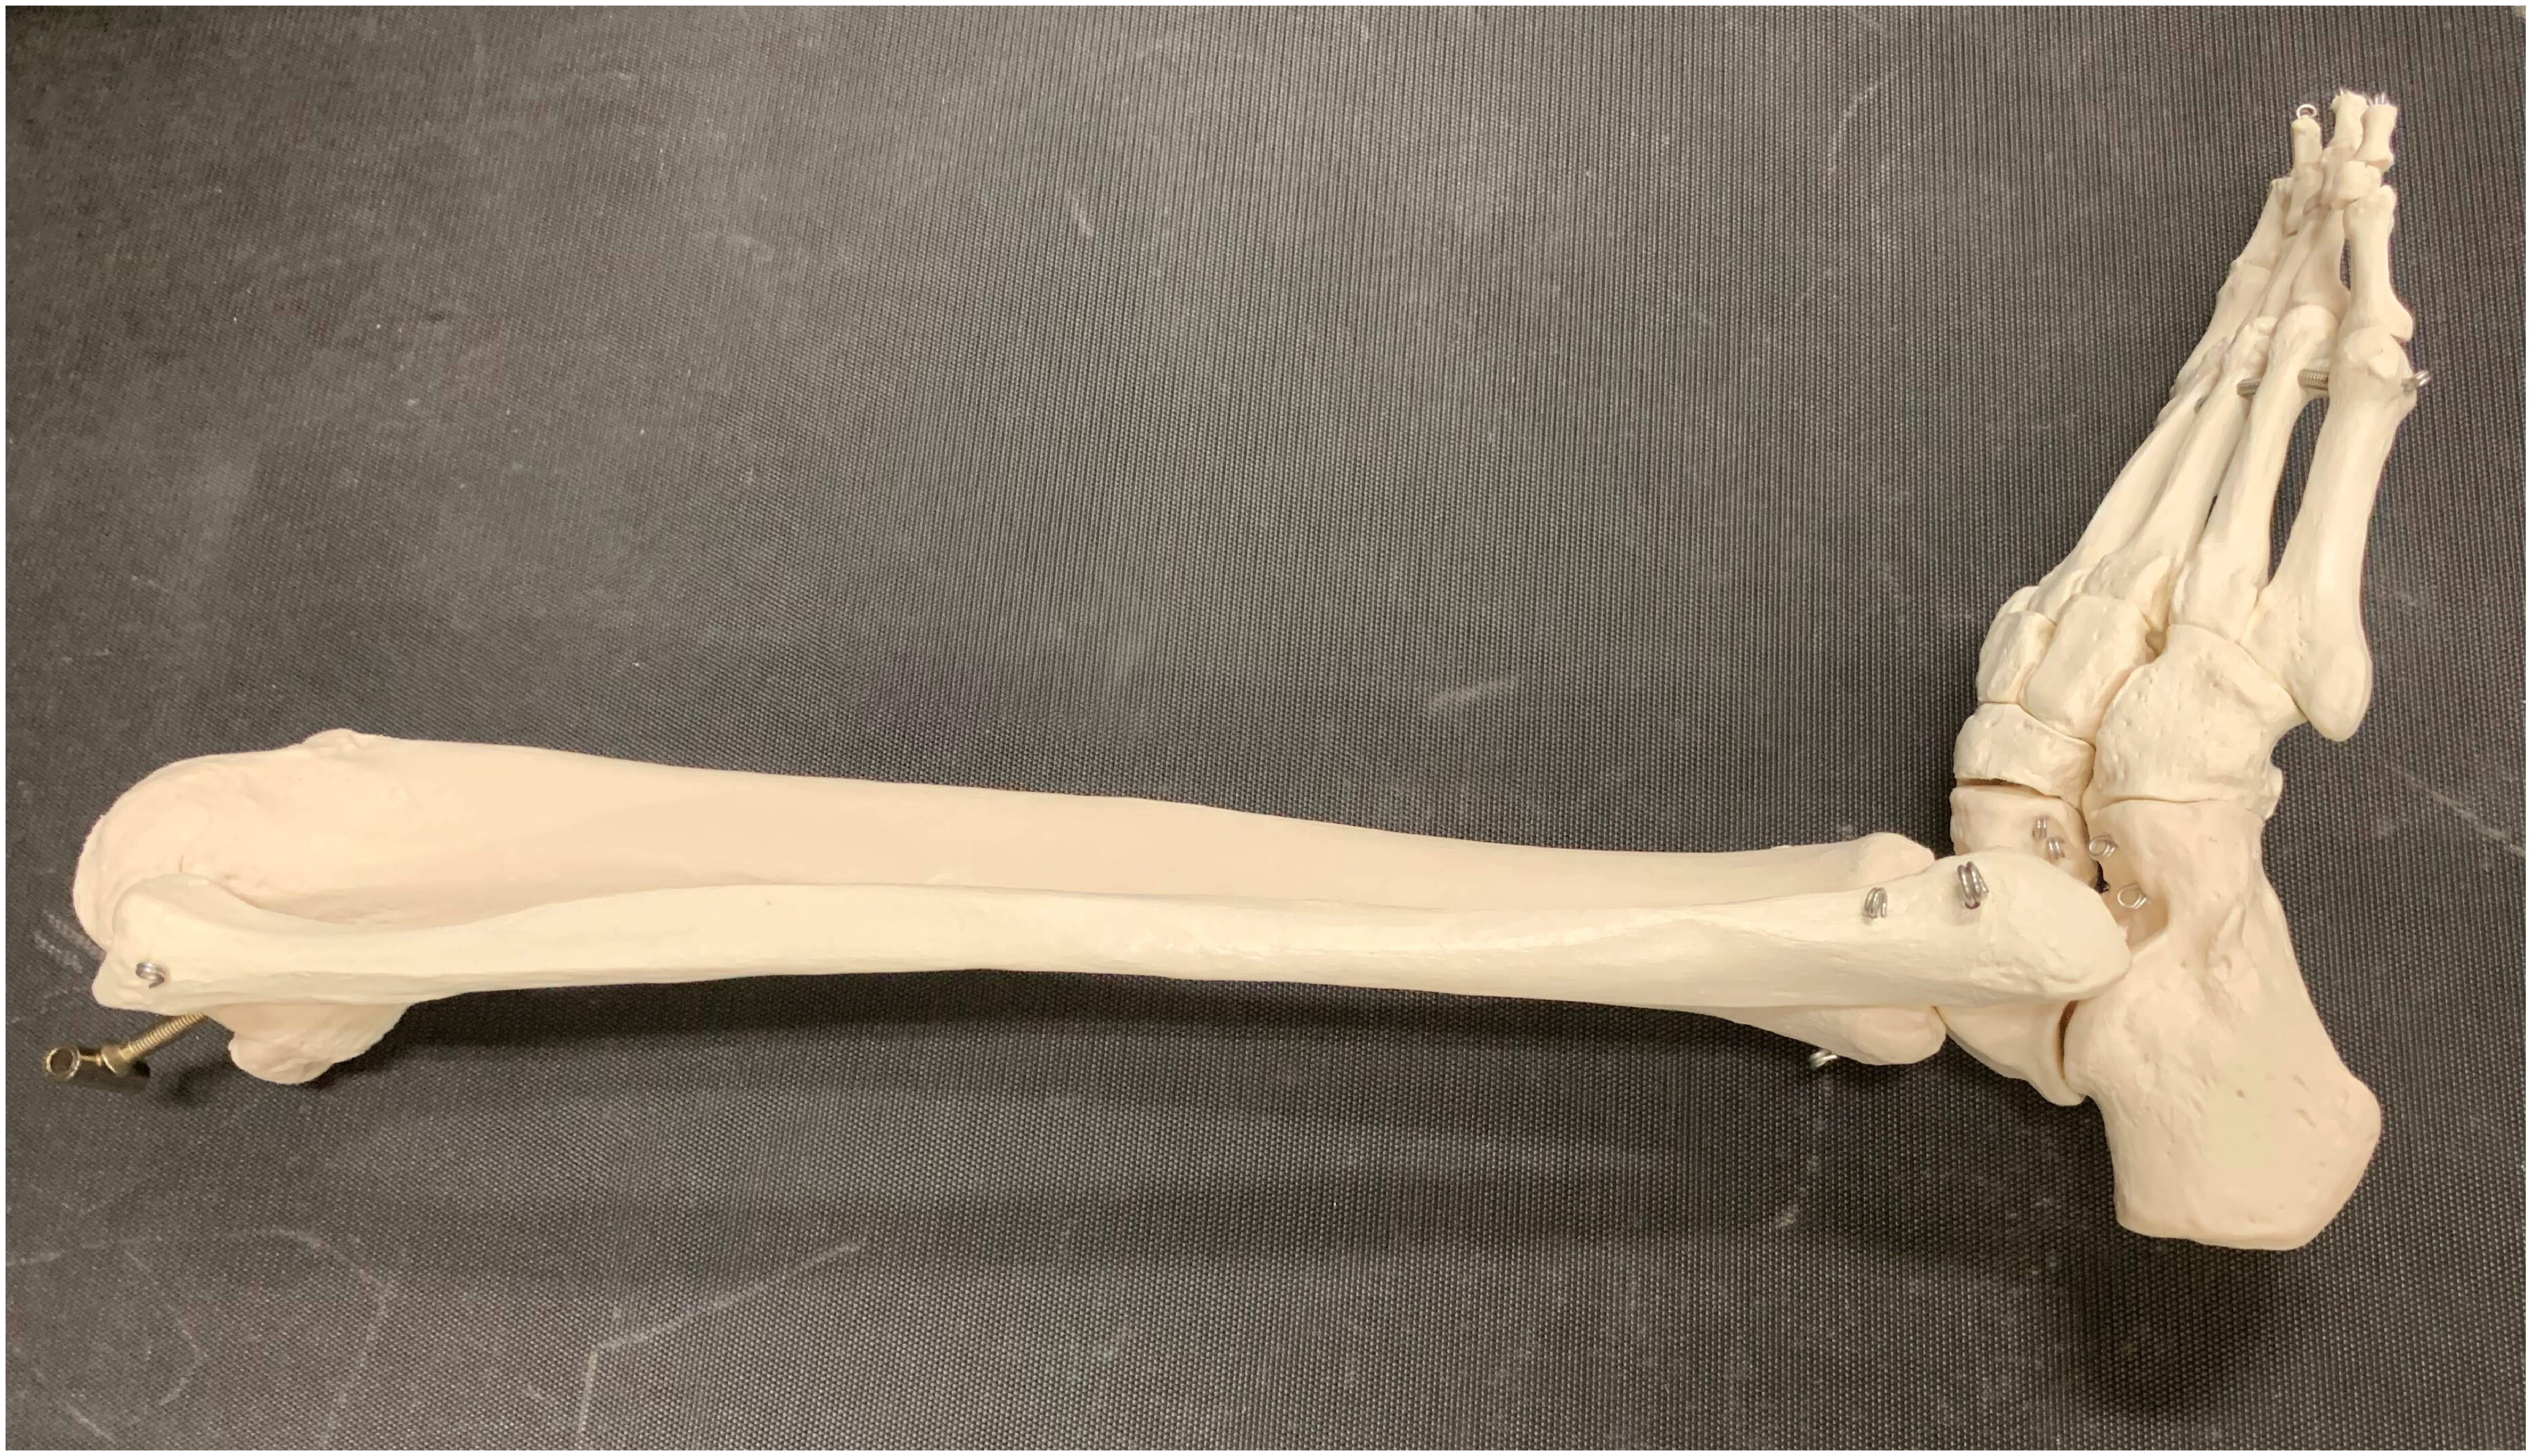
\includegraphics[width=0.6\columnwidth,clip]{./2_measurement/legBone.eps}
     \caption{人体模型骨格(脚部)}
     \label{fig:legBone}
    \end{center}
\end{figure}
\newpage
以前製作されたペダリングロボット,2足歩行ロボットでは関節部分にピンジョイントを用いていたが,今回製作する足関節ロボットでは,
自由度を向上させることを一つの目的としているので,膝部分にピンジョイント,足首部分にボールジョイントを用いた.

まず初めに前脛骨筋の両端を彫刻刀やバンドソーを用いて平面を作成した.続いてそこに,ボルト/ナットを用いてボールジョイント,ピンジョイントの軸受けの
固定を行った.そして,人間の筋付着位置に合わせて空気圧人工筋を接続するため,リングボルトを設置した.その結果,下記のFig.\ref{fig:legJoint}の様になった.

\begin{figure}[h]
    \begin{center}
     
\includegraphics[width=0.6\columnwidth,clip]{./2_measurement/legJoint.eps}
     \caption{ジョイント,リングボルト接地状態(脚部)}
     \label{fig:legJoint}
    \end{center}
\end{figure}
次に重心位置を人間のものと合わせ,重量を成人男性の1/2にする作業を行った.
人体模型の骨は樹脂でできているため軽量であるので,鉛シートを巻き調整を行った.
重心位置の確認には紐で巻いて垂らし,その鉛直線が交わるところで求めた.
重量,重心位置の調整を行った結果,Fig.\ref{fig:legPb}の様になった.

\begin{figure}[h]
    \begin{center}
     
\includegraphics[width=0.6\columnwidth,clip]{./2_measurement/legPb.eps}
     \caption{鉛シートを巻いた結果}
     \label{fig:legPb}
    \end{center}
\end{figure}
\newpage
続いて,足の製作を行った.前脛骨筋と同様に,人間の筋付着位置に合わせて空気圧人工筋の
接続をするリングボルトの設置をした.また,補強用として足の裏部分にアルミ板を固定した.
そして,ボールジョイント接続部分に穴をあけタップドリルを用いてねじ溝を掘った.

\begin{figure}[h]
    \begin{center}
     
\includegraphics[width=0.6\columnwidth,clip]{./2_measurement/foot.eps}
     \caption{リングボルト設置結果(足上面)}
     \label{fig:foot}
    \end{center}
\end{figure}
\begin{figure}[h]
    \begin{center}
     
\includegraphics[width=0.6\columnwidth,clip]{./2_measurement/footside.eps}
     \caption{リングボルト設置結果(足側面)}
     \label{fig:footside}
    \end{center}
\end{figure}

\newpage
その後,指先と踵の間を丁番を用いて接続し,ピッチ方向に自由度を持たせた.その結果,Fig.\ref{fig:foot2},\ref{fig:footside2}の様になった.
なお,空気圧人工筋などの能動的なアクチュエータは用いず,接地時に可動する受動的なものとして用いる様にした.
そして,その足にシリコン材を用いて肉付けを行い,重量,重心位置の調整をおこなった.
この時,脛骨と同様に重心位置は成人男性,重量は成人男性の1/2となるように調整をおこなった.
なお,脛骨と異なり鉛シートを用いずシリコン材を用いたのは衝撃吸収と成型性のしやすさからその様にした.
\begin{figure}[h]
    \begin{center}
     
\includegraphics[width=0.6\columnwidth,clip]{./2_measurement/siliconfoot.eps}
     \caption{シリコン材,丁番設置結果(足上面)}
     \label{fig:foot2}
    \end{center}
\end{figure}
\begin{figure}[h]
    \begin{center}
     
\includegraphics[width=0.6\columnwidth,clip]{./2_measurement/siliconfootside.eps}
     \caption{シリコン材,丁番設置結果(足側面)}
     \label{fig:footside2}
    \end{center}
\end{figure}
\newpage
続いて,脛骨と足部をボールジョイントのねじを用いて接続した.そして,人間の前脛骨筋,長腓骨筋,ヒラメ筋にあたる
空気圧人工筋3本を,それぞれワイヤーを用いてリングボルトと接続した.最後に,足部に靴を履かせて完成した.
完成したものは,Fig.\ref{fig:fin}である.

\begin{figure}[h]
    \begin{center}
     
\includegraphics[width=0.6\columnwidth,clip]{./2_measurement/fin.eps}
     \caption{完成した足関節ロボット}
     \label{fig:fin}
    \end{center}
\end{figure}
\chapter{計測・実験手法}
\section{計測手法}
\subsection{ストレッチセンサ計測アルゴリズム}
\ref{sec:RC回路}にて示す通り,ストレッチセンサの静電容量変化の計測にはRC回路を用いた時定数の計測で行った.
なお,この時定数の計測にはNucleoF303K8といったマイコン評価ボードを使用した.また,それらのコードの記述にはmbedライブラリを使用した.
使用したソースコードは下記リンクにて公開している.計測アルゴリズムはFig.\ref{fig:algorithm}にて示すように
1000Hzで計測を実行し,100Hzごとに計測データの平均値をSerial通信を用いてPCに出力した.
また,2000Hzで出力ピンの状態を切り替え,ストレッチセンサに電荷が残らないようにした.

ソースコード:https://os.mbed.com/users/HidetoN/code/Cap-Sensor/

\begin{figure}[h]
    \begin{center}
     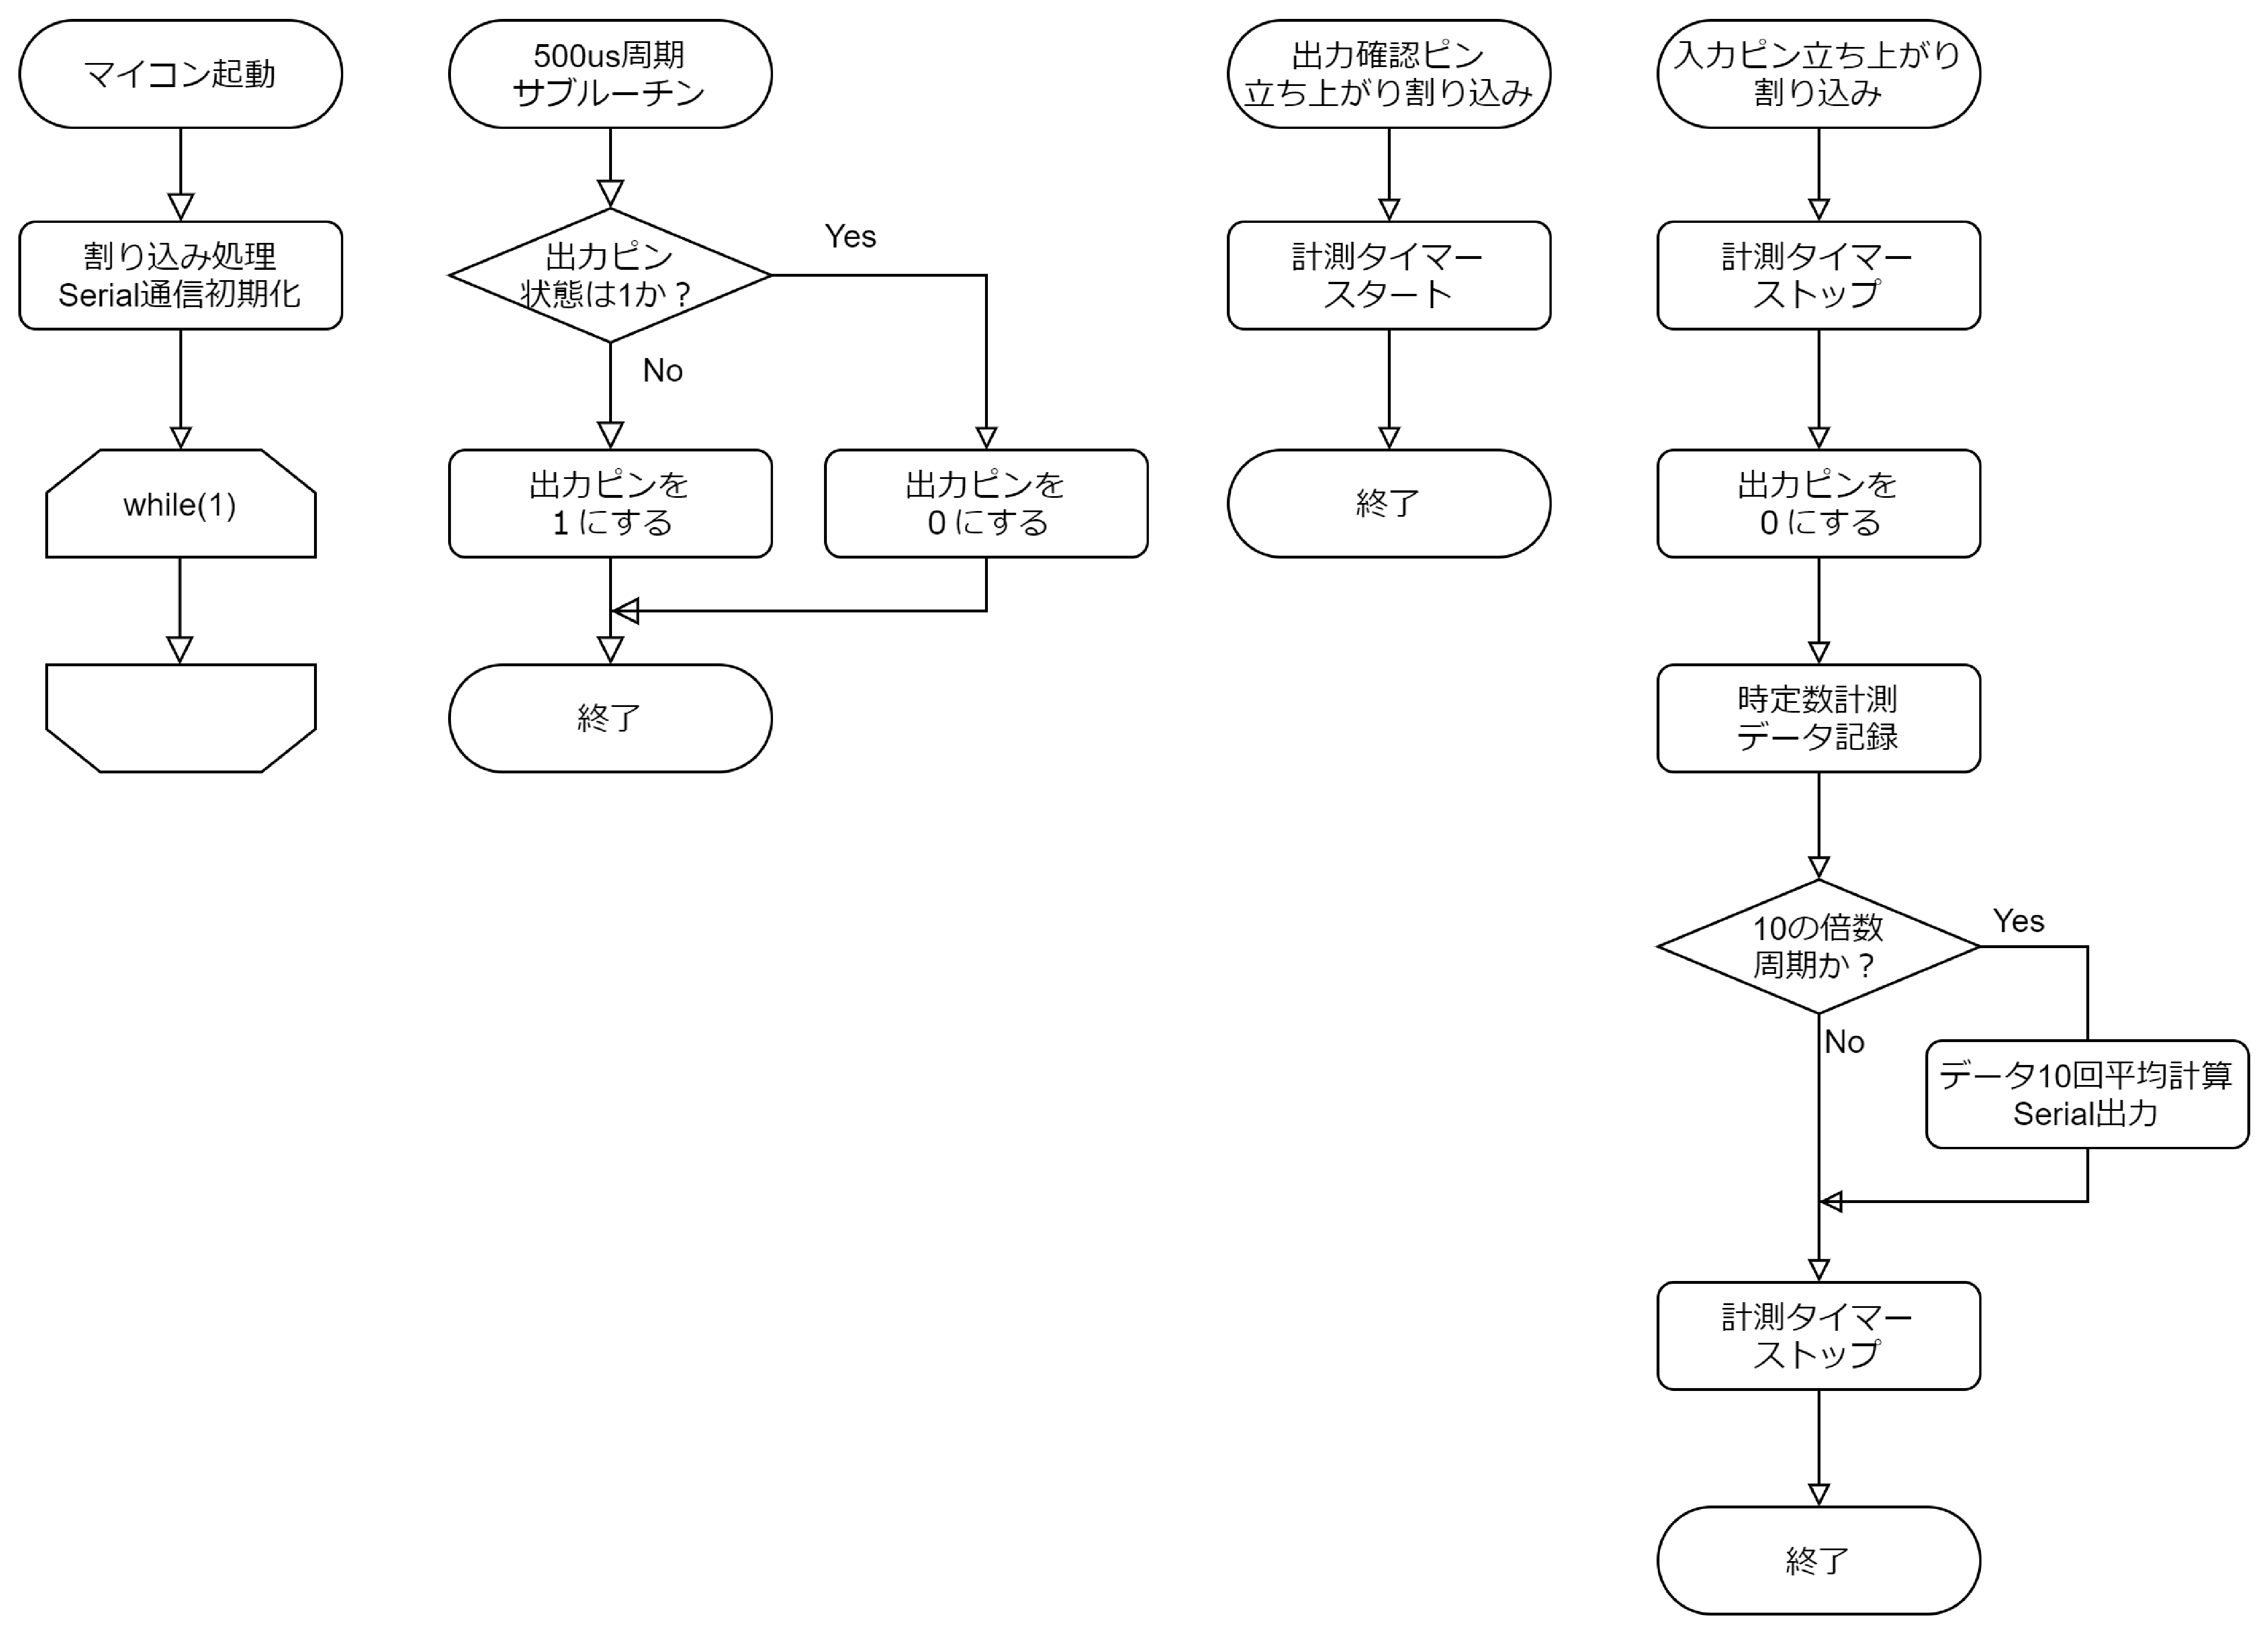
\includegraphics[width=0.9\columnwidth,clip]{./3_analysis/algorithm.eps}
     \caption{計測プログラムにおけるアルゴリズム}
     \label{fig:algorithm}
    \end{center}
\end{figure}

\subsection{ストレッチセンサ計測システム}
ストレッチセンサの計測データはNucleoF303K8よりSerial通信によって921600bpsで出力される.
制御アルゴリズムの部分でも示したが,1000Hz周期で取得したデータの平均値が100Hz周期に出力される.
このデータをTeraTermのログ取得機能を用いてcsvファイルとして保存した.
なお,足関節ロボット制御用PCの処理の都合上,別PCを用いて結果の取得を行った.
\begin{figure}[h]
    \begin{center}
        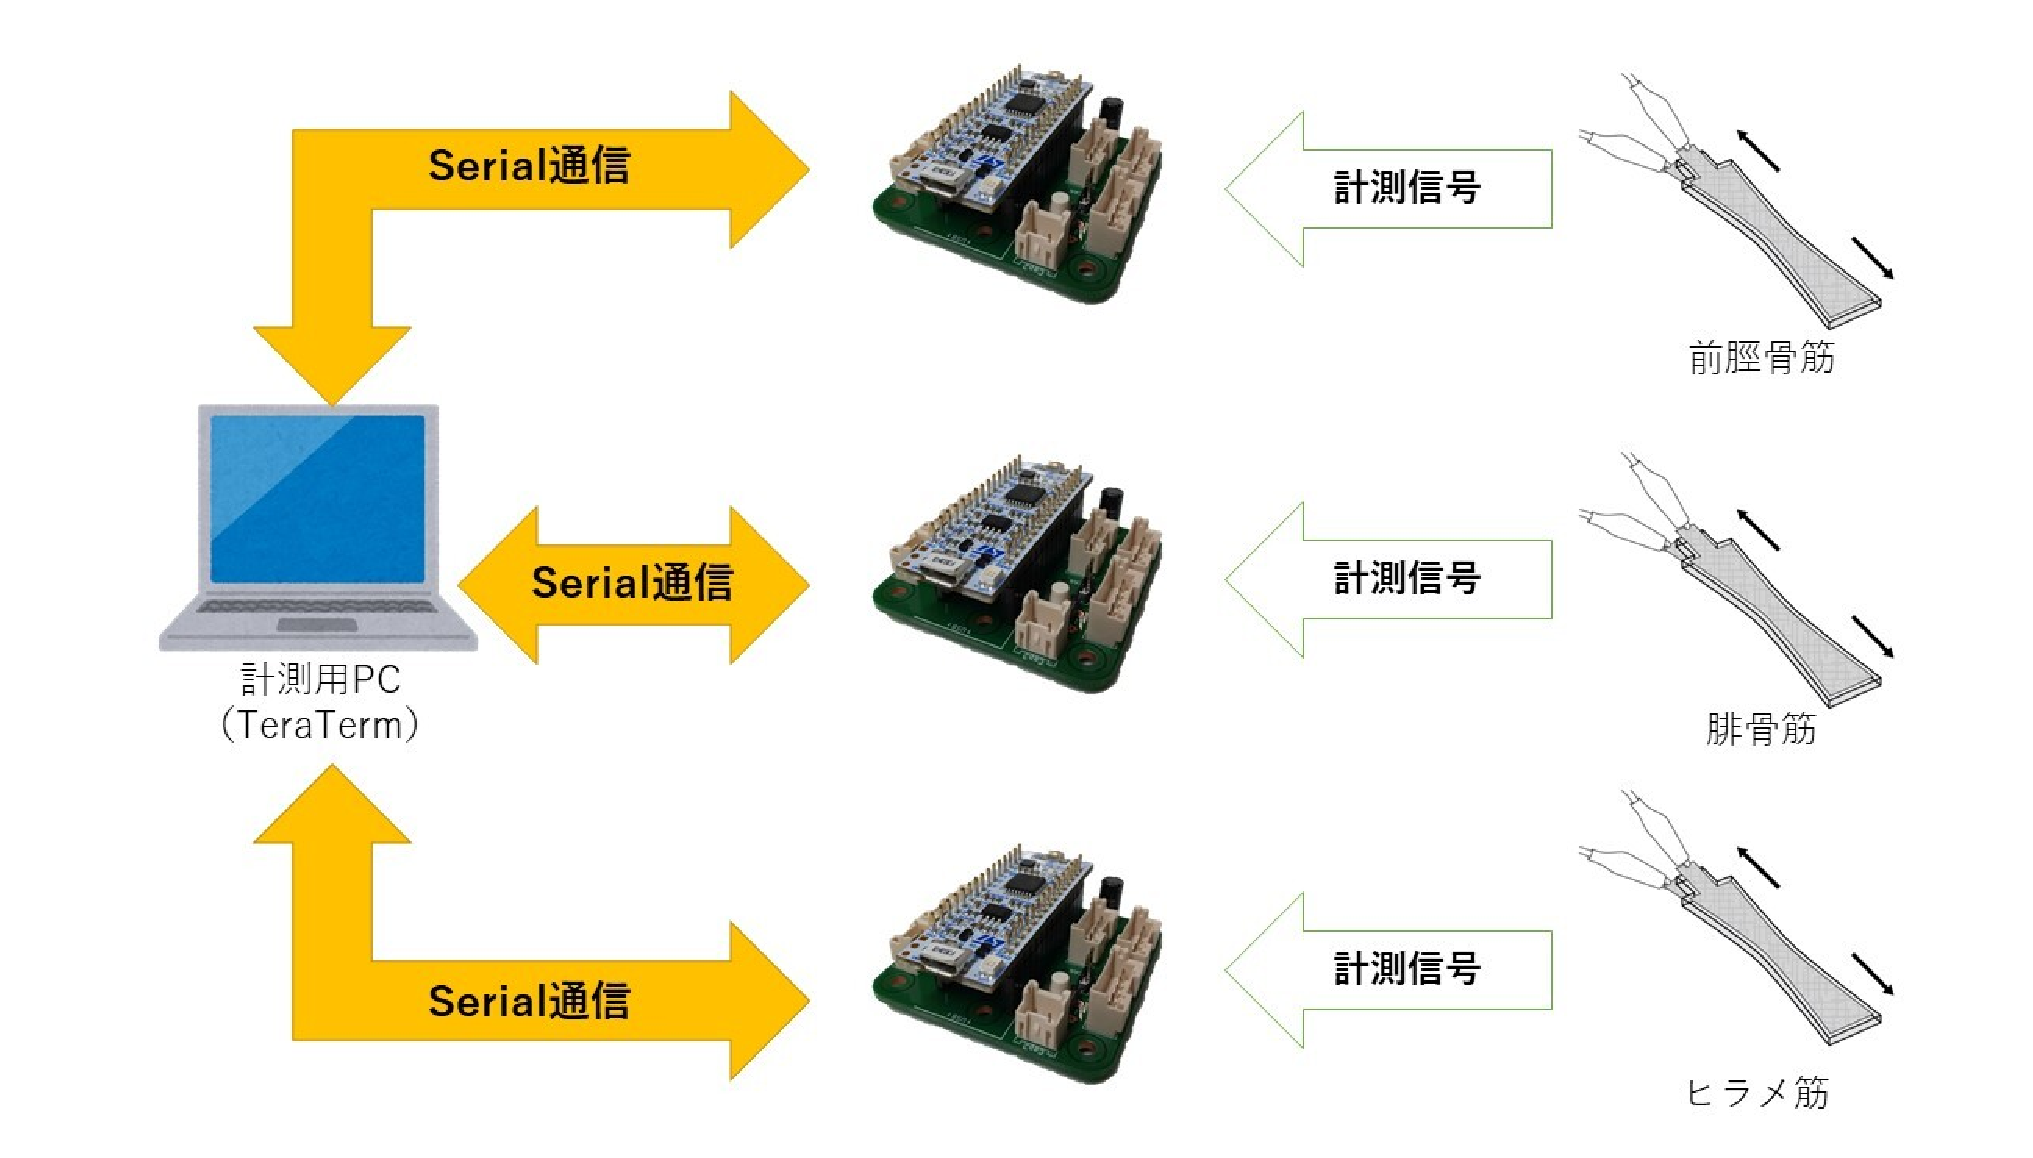
\includegraphics[width=0.78\columnwidth,clip]{./3_analysis/getSystem.eps}
        \caption{計測システム概略図}
        \label{getSystem}
    \end{center}
\end{figure}

\subsection{足関節ロボット駆動システム}
足関節ロボットの駆動システムには従来から存在するペダリングロボット,2足歩行ロボットのシステムと同様のシステムを利用した.
以下にそのシステムに関して記述する.

まず,Fig.\ref{fig:compressor}にて示す,エアーコンプレッサーで8気圧まで圧縮空気を作成し,気圧調整弁を用いて6気圧まで減圧を行った.
続いて,制御用PCに搭載されたDAボードより,空気圧制御盤にアナログ信号を送信する.なお,この電圧指令は550段階で制御が行うことが出来る.
この電圧指令を元に空気圧制御盤に搭載された空気圧制御器によって可変的に空気圧の制御を各人工筋に対して行う.

\newpage

\begin{figure}[h]
    \begin{center}
     
\includegraphics[width=0.65\columnwidth,clip]{./3_analysis/compressor.eps}
     \caption{使用したエアーコンプレッサー}
     \label{fig:compressor}
    \end{center}
\end{figure}

\begin{figure}[h]
    \begin{center}
     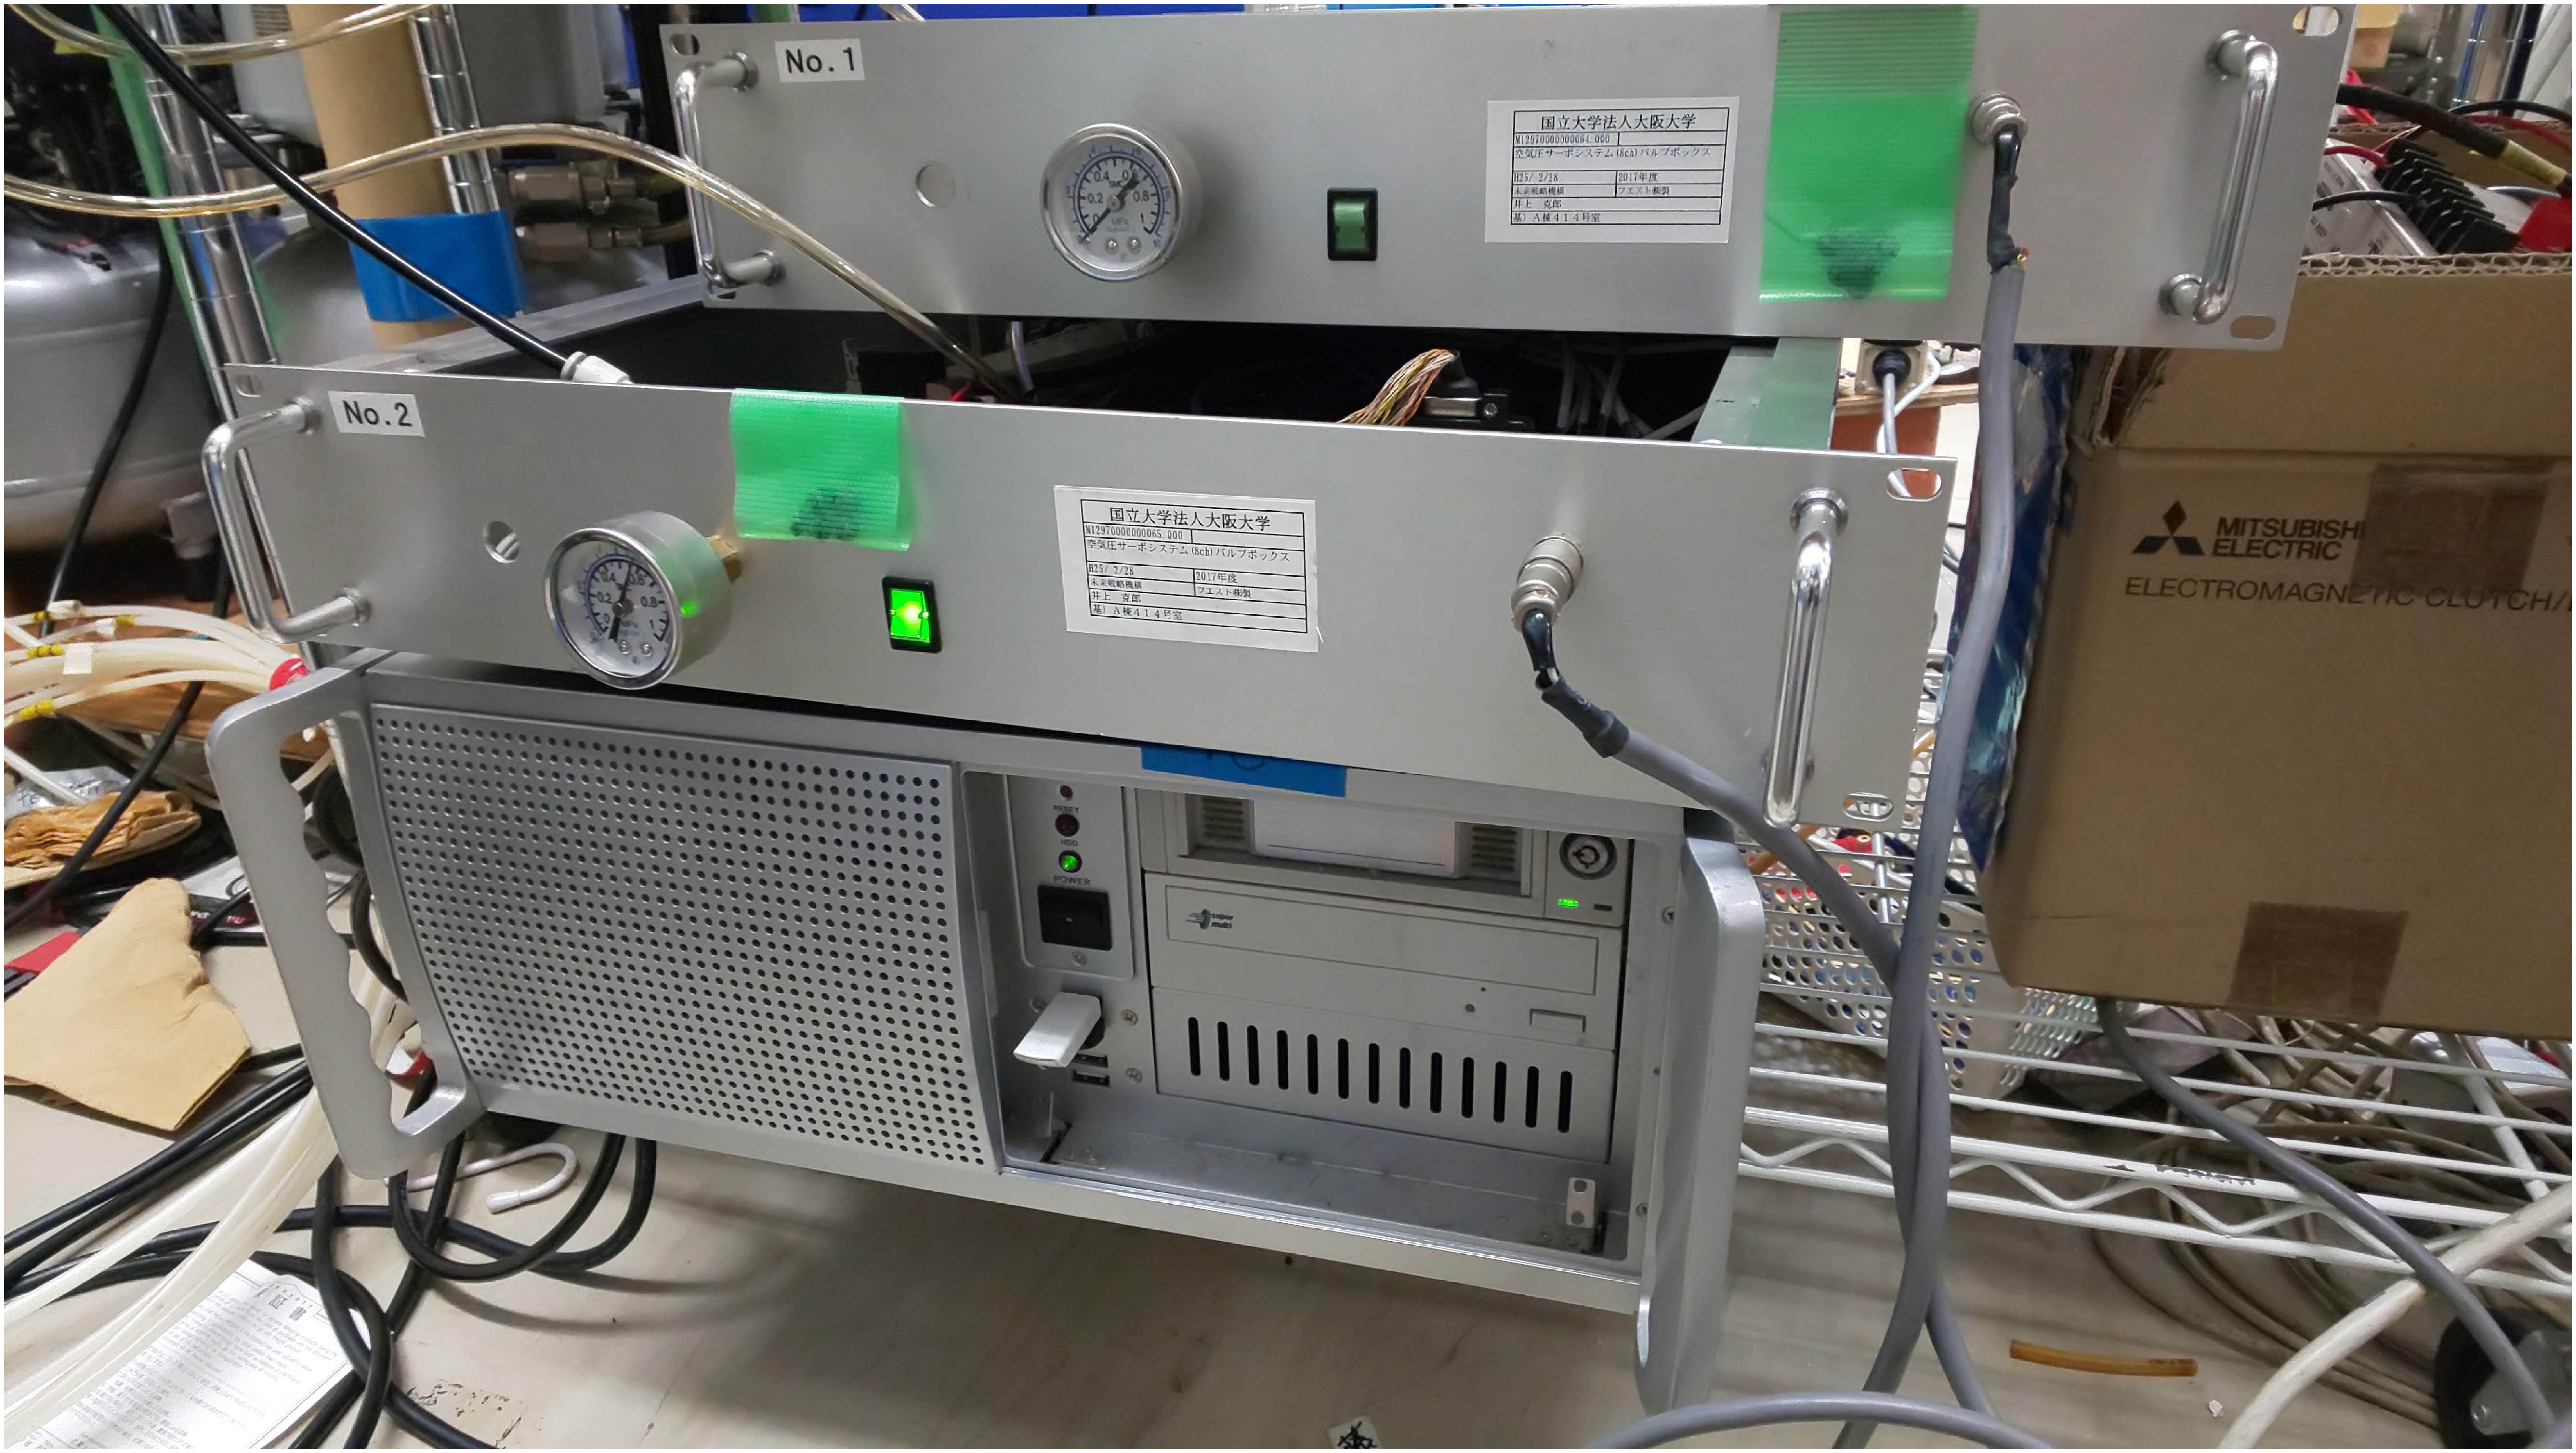
\includegraphics[width=0.65\columnwidth,clip]{./3_analysis/PC.eps}
     \caption{制御PCとエアー制御盤}
     \label{fig:PC}
    \end{center}
\end{figure}

\newpage

\section{実験手法}
\subsection{ストレッチセンサ計測精度評価}
今回製作した,ストレッチセンサの精度評価として各空気圧人工筋にsin出力を段階的に与えて,センサの計測値と,実際の長さの比較を行った.
実際の長さの計測は,ノギスを用いて計測を行った.与えた出力値は12段階とした.底背屈動作をモデルに検討を行うため,前脛骨筋と腓骨筋/ヒラメ筋の
組み合わせで出力を与えることとした.Fig.\ref{output_for_test}に示す様な出力を各空気圧人工筋に対して与えた.

センサでの時定数計測に関して,計測値を安定させるため30秒ほど記録を行った.
そしてその後,サンプル数$n$,計測値$t_i \left(i=0,1,\cdots,n\right)$としたとき,
\begin{eqnarray}
        \overline{t}=\frac{\sum_{i=0}^n t_i}{n}
        \label{ave}
\end{eqnarray}
といった式で求まる,総和平均$\overline{t}$を用いて時定数を求めた.
また,その誤差$\delta t$として,
\begin{eqnarray}
    \delta t = \sqrt{ \frac{\sum_{i=0}^n \left(t_i-\overline{t}\right)^2}{n(n-1)}}
    \label{std}
\end{eqnarray}
といった式で求まる,標準誤差を用いて計算した.

\begin{figure}[h]
    \begin{center}
        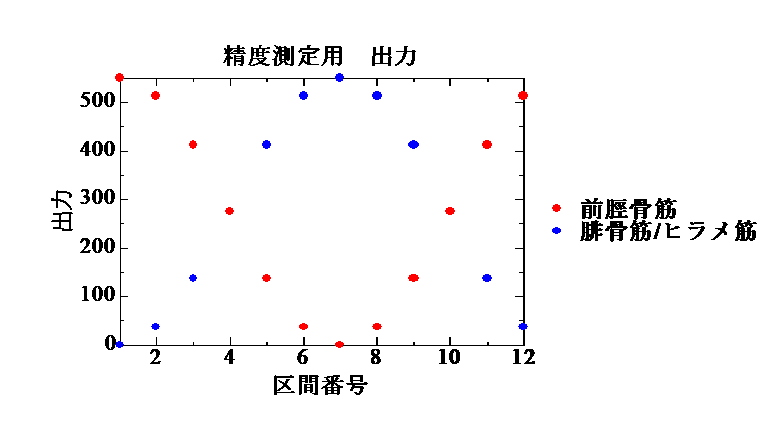
\includegraphics[width=0.76\columnwidth,clip]{2_measurement/output/output.eps}
        \caption{精度評価用 出力}
        \label{output_for_test}
    \end{center}
\end{figure}

\newpage

\subsection{ストレッチセンサ動的計測}
上記で計測した結果を元に,足関節ロボットに1Hzのsin周期運動をさせ,ストレッチセンサを用いて各筋の伸長計測を行った.
なお,各筋に与える出力はFig.\ref{output_for_actions}に示すものを与えた.

\begin{figure}[h]
  \begin{center}
  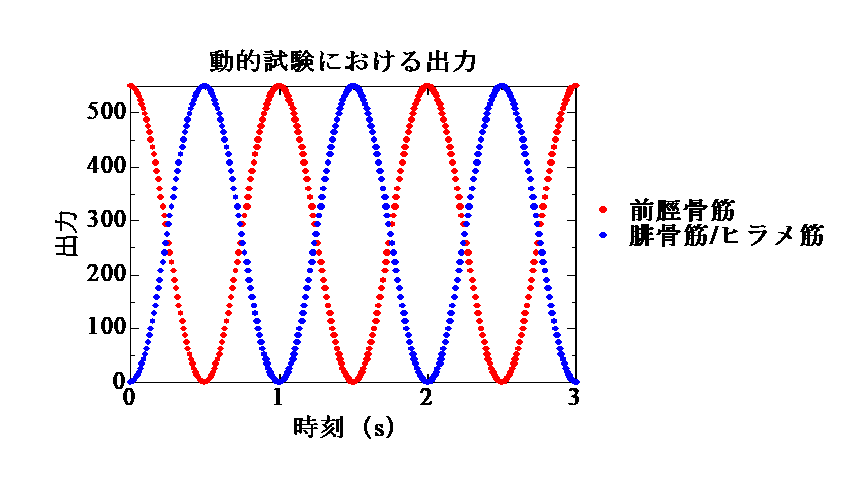
\includegraphics[width=0.76\columnwidth,clip]{3_analysis/outPut/putPut.eps}
  \caption{動的計測}
  \label{output_for_actions}
  \end{center}
\end{figure}

解析方法として,与えた出力が1Hzであること,データの出力周期が100Hzであることを用いて,
1秒ごとに区切り0.01秒ごとの区間の平均値,標準誤差の計算を行った.
なお,それぞれの計算には式\ref{ave},\ref{std}をそれぞれ用いた.

\chapter{結果・考察}
\section{結果}
\subsection{ストレッチセンサ計測精度評価}
Fig. \ref{output_for_test}のような出力を各空気圧人工筋に与えた結果,
Table.\ref{strain}のような長さの結果となった.
また,それぞれの時におけるストレッチセンサ時定数の結果を求めると,Table.\ref{4_2}に示す様になった.
\begin{table}[h]
    \caption{ストレッチセンサ 長さ(mm) 計測結果}
    \label{strain}
    \begin{center}
        \begin{tabular}{|c|c|ccc|}\hline
            \multicolumn{2}{|c|}{} & \multicolumn{3}{c|}{筋肉種類}\\
            \cline{3-5}
            \multicolumn{2}{|c|}{} & 前脛骨筋 & 腓骨筋 & ヒラメ筋 \\ \hline
            & 1 & 236 & 194 & 208 \\ \cline{2-5}
            & 2 & 234 & 197 & 210 \\ \cline{2-5}
            & 3 & 233 & 198 & 213 \\ \cline{2-5}
            & 4 & 234 & 199 & 214 \\ \cline{2-5}
            & 5 & 220 & 204 & 215 \\ \cline{2-5}
            計測位置 & 6 & 208 & 217 & 225 \\ \cline{2-5}
            & 7 & 214 & 217 & 227 \\ \cline{2-5}
            & 8 & 215 & 215 & 223 \\ \cline{2-5}
            & 9 & 218 & 203 & 218 \\ \cline{2-5}
            & 10 & 233 & 195 & 216 \\ \cline{2-5}
            & 11 & 234 & 192 & 212 \\ \cline{2-5}
            & 12 & 235 & 197 & 209 \\ \hline
        \end{tabular}
    \end{center}
\end{table}

\newpage

%セルを結合して中央揃え
%(参考):https://qiita.com/ta_b0_/items/c8c828b6a53d49498736
\begin{table}[h]
    \caption{ストレッチセンサ 時定数(us) 計測結果}
    \label{4_2}
        \begin{center}
            \begin{tabular}{|c|c|ccc|}\hline
            \multicolumn{2}{|c|}{} & \multicolumn{3}{c|}{筋肉種類}\\
            \cline{3-5}
            \multicolumn{2}{|c|}{} & 前脛骨筋 & 腓骨筋 & ヒラメ筋 \\ \hline
            & 1 & 43.86±0.02 & 68.14±0.03 & 40.13±0.01 \\ \cline{2-5}
            & 2 & 44.42±0.02 & 68.07±0.02 & 40.13±0.01 \\ \cline{2-5}
            & 3 & 44.73±0.02 & 68.07±0.02 & 39.26±0.01 \\ \cline{2-5}
            & 4 & 44.50±0.01 & 67.12±0.04 & 38.43±0.02 \\ \cline{2-5}
            & 5 & 46.74±0.01 & 66.86±0.02 & 38.45±0.01 \\ \cline{2-5}
            計測位置 & 6 & 46.93±0.02 & 63.37±0.01 & 37.24±0.01 \\ \cline{2-5}
            & 7 & 47.03±0.01 & 64.74±0.05 & 37.33±0.01 \\ \cline{2-5}
            & 8 & 47.02±0.01 & 64.76±0.03 & 37.17±0.01 \\ \cline{2-5}
            & 9 & 46.80±0.01 & 65.92±0.03 & 37.38±0.01 \\ \cline{2-5}
            & 10 & 44.20±0.01 & 66.76±0.04 & 38.21±0.01 \\ \cline{2-5}
            & 11 & 44.74±0.01 & 66.92±0.05 & 38.46±0.01 \\ \cline{2-5}
            & 12 & 45.13±0.02 & 66.90±0.03 & 38.65±0.01 \\ \hline
        \end{tabular}
    \end{center}
\end{table}

\subsection{ストレッチセンサ動的計測}

Fig. \ref{output_for_actions}のような出力を各空気圧人工筋に与え,
1秒ごとに区切り0.01秒ごとの区間の平均値,標準誤差の計算を行った結果,
Fig.\ref{zenkei_action},\ref{hikotsu_action},\ref{hirame_action}に示すようになった.
\begin{figure}[h]
  \begin{center}
  \includegraphics[width=0.75\columnwidth,clip]{./4_consideration/moving/zenkei.eps}
  \caption{ストレッチセンサ動的計測結果(前脛骨筋)}
  \label{zenkei_action}
  \end{center}
\end{figure}
\begin{figure}[h]
  \begin{center}
  \includegraphics[width=0.75\columnwidth,clip]{./4_consideration/moving/hikotsu.eps}
  \caption{ストレッチセンサ動的計測結果(腓骨筋)}
  \label{hikotsu_action}
  \end{center}
\end{figure}

\clearpage

\begin{figure}[h]
  \begin{center}
  \includegraphics[width=0.75\columnwidth,clip]{./4_consideration/moving/hirame.eps}
  \caption{ストレッチセンサ動的計測結果(ヒラメ筋)}
  \label{hirame_action}
  \end{center}
\end{figure}

\section{考察}
\subsection{ストレッチセンサ計測精度}
先ほどの結果より,それぞれの計測位置における空気圧人工筋の長さをグラフに表すと,
Fig.\ref{4-ml}の様になった.このグラフから見てわかるように,腓骨筋とヒラメ筋が組となって
前脛骨筋と逆位相のsin波形的動きをさせることが出来た.今回,足関節ロボットの空気圧人工筋
それぞれに対して,Fig.\ref{output_for_test}の出力を出すよう指令を与えたので
システムとして問題なく動いたことがわかった.

続いて,Table.\ref{4_2}の結果を用いて,横軸にセンサの長さ,縦軸に時定数としたグラフを
描画すると,Fig.\ref{ml-rc1},\ref{ml-rc2},\ref{ml-rc3}に示すようになった.
各筋肉に関して,長さが増加するとセンサでの計測値が減少した.
どの筋肉においても同様の結果を示しており,ストレッチセンサが伸びると
静電容量が減少するといったことが分かった.

一方でセンサごとに空気圧人工筋の長さに対する計測値の変化の特性が異なる.これは,
センサ自体が自作されており,その製作時のむらによるものだと考えられる.それに加えて,
空気圧人工筋に設置する時にある程度テンションを与えて設置するのだが,そのテンションの
かけ方具合にもよると考えられる.実際に使用するときは,ストレッチセンサを空気圧人工筋に
設置した状態で,今回の実験の様にセンサ特性の解析を行う必要があると考えられる.

また,空気圧人工筋の伸びの変化に対して,時定数の変化が非常に微小なものとなっている.
今回の時定数の結果や,製作したRC回路の抵抗値$1.5M\Omega$より静電容量の変化量に関して考えると,
最も変化が大きかった腓骨筋においても$42~45pF$の変化しか現れなかった.
これに対する対策として,RC回路における抵抗値の再選定を行う必要があると考えられた.
抵抗値を増加させると時定数も増加するのでマイコンで変化量を計測しやすくなる.
一方で,抵抗値を増大させると計測ノイズ成分も大きくなるので,その辺りも踏まえて抵抗値の
再選定をしていく必要があると考えられる.

\begin{figure}[h]
    \begin{center}
        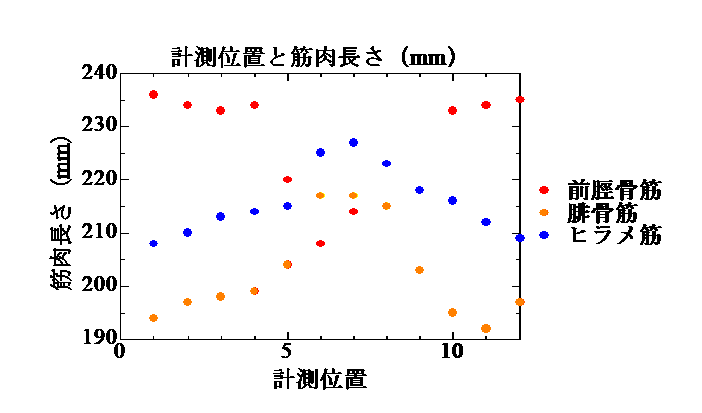
\includegraphics[width=0.7\columnwidth,clip]{4_consideration/ml.eps}
    \end{center}
    \caption{計測位置と各空気圧人工筋の長さの関係}
    \label{4-ml}
\end{figure}

\begin{figure}[h]
    \begin{center}
        \includegraphics[width=0.7\columnwidth,clip]{4_consideration/zenkei.eps}
    \end{center}
    \caption{空気圧人工筋の長さとセンサ計測値の関係(前脛骨筋)}
    \label{ml-rc1}
\end{figure}
\clearpage
\begin{figure}[h]
    \begin{center}
        \includegraphics[width=0.7\columnwidth,clip]{4_consideration/hikotsu.eps}
    \end{center}
    \caption{空気圧人工筋の長さとセンサ計測値の関係(腓骨筋)}
    \label{ml-rc2}
\end{figure}
\begin{figure}[h]
    \begin{center}
        \includegraphics[width=0.7\columnwidth,clip]{4_consideration/hirame.eps}
    \end{center}
    \caption{空気圧人工筋の長さとセンサ計測値の関係(ヒラメ筋)}
    \label{ml-rc3}
\end{figure}
\clearpage
\subsection{ストレッチセンサ動的計測}
今回,各筋肉に1Hzの周期動作を入れ,区間ごとに区切り各平均値の計算を行った.
おおむね,各筋において計測精度評価にて観測された時定数内に収まっていた.これは,
ストレッチセンサを用いた,筋肉の伸縮計測において,再現性があると考えられる.
また,静的にストレッチセンサの実長さの計測を行った上で,ストレッチセンサを用いて
時定数の計測を行うと,実長さが算出できることが分かった.

一方で,今回足関節ロボットの空気圧人工筋動作システムとストレッチセンサの計測システムが,
実装の仕様上,同一システム上となっていないので,足関節ロボットが動作している途中からの
ストレッチセンサの計測となった.このことにより,ストレッチセンサの計測開始と,
空気圧人工筋の出力開始とが合っていない状態となってしまった.
また,計測システムの都合上それぞれのストレッチセンサに対して独立に計測を行ったため,
それぞれのストレッチセンサの計測開始位置も合っていない状態となっている.

上記のことを補正するため,前脛骨筋に関しては時定数の最小値を,腓骨筋,ヒラメ筋に関して最大値を
0秒として処理した.このように処理した理由として,Fig.\ref{output_for_actions}にて示す
出力を各空気圧人工筋に与えたこと,また,Fig.\ref{ml-rc1},\ref{ml-rc2},\ref{ml-rc3}に示す
ように,空気圧人工筋の実長さに対して,時定数は単調減少となってことが元となっている.
これらの結果より,周期位置の補正結果はFig.\ref{min-rc1},\ref{min-rc2},\ref{min-rc3}に示すようになった.
また,それぞれの筋における周期時刻補正後の時定数最小値/最大値の周期時刻は下記の Table.\ref{min-max}に
示すようになった.これらの結果より,背屈方向にかかる時間よりも底屈方向にかかる時間の方が長いことが分かった.
本来であれば,1Hzのsin動作であり,底屈動作,背屈動作ともに0.5sで行われるべき動作である.
これは,重力の影響により,底屈動作よりも背屈動作の方が行われやすかったからと考えられる.
これらの確認として,実際に空気圧人工筋に与えている出力とストレッチセンサの時定数の関係を調べる必要があるとも考えられる.
\begin{table}[h]
  \begin{center}
    \label{min-max}
    \caption{周期時刻補正後の時定数最大値/最小値における周期時刻}
    \begin{tabular}{|c||c|c|c|}\hline
      & 前脛骨筋 & 腓骨筋 & ヒラメ筋 \\ \hline \hline
      最小値 & 0.00s & 0.27s & 0.31s \\ \hline
      最大値 & 0.43s & 0.00s & 0.00s \\ \hline
    \end{tabular}
  \end{center}
\end{table}

\begin{figure}[h]
    \begin{center}
        \includegraphics[width=0.75\columnwidth,clip]{4_consideration/min/zenkei.eps}
    \end{center}
    \caption{動的計測 補正結果(前脛骨筋)}
    \label{min-rc1}
    \begin{center}
        \includegraphics[width=0.75\columnwidth,clip]{4_consideration/min/hikotsu.eps}
    \end{center}
    \caption{動的計測 補正結果(腓骨筋)}
    \label{min-rc2}
\end{figure}
\begin{figure}[t]
    \begin{center}
        \includegraphics[width=0.75\columnwidth,clip]{4_consideration/min/hirame.eps}
    \end{center}
    \caption{動的計測 補正結果(ヒラメ筋)}
    \label{min-rc3}
\end{figure}

\chapter{結言}
本研究では,ヒトと同じ自由度を持った足関節ロボット,伸縮性に富んだフレキシブルストレッチセンサ
(ストレッチセンサ)の開発製作を行った.

足関節ロボットにおいて従来では底背屈動作しか行うことが出来なかったものが,ヒトの足関節と同様の
自由度を持った3自由度の動きをすることが,可能になった.また,この自由度で動作することを
,腓骨筋とヒラメ筋,前脛骨筋の組み合わせで動作させ確認することができた.

現在,足関節ロボットは左足のみであるが既存の2足歩行ロボットの様に両足を備えた骨盤より下の
下肢ロボットになるよう製作を行っていく必要があると思われる.これによって実際のヒトと同じ
自由度を持った空気圧人工筋を用いた2足歩行ロボットとなり,ヒトの運動戦略の解析に役立つと
考えられる為である.

ストレッチセンサにおいて,実際に計測回路も含めて製作し空気圧人工筋に搭載した.そして,
空気圧人工筋の伸縮に関して計測を行うことが出来た.また,周期動作を行っている空気圧人工筋の
伸縮に関して計測を行うこともできた.既製品では5万円程かかる所を,
計測回路も含め6千円程度で製作した.これにより,安価に多チャンネルの計測を行うことができる
様になった.

今後の課題として,ストレッチセンサのさらなる実用化を行っていく必要があると思われる.具体的には,
ロボットの制御系にストレッチセンサの計測系を組み込み,フィードバック系として活用できる様に
することが一つとして挙げられる.これに備えて,現在では計測後にデータ処理等を行っていたが,
リアルタイムにデータ処理を行えるように組む必要性があると考えられる.また,現在は製作したセンサごとの
特性のばらつきが大きいが定量的に製作できるようにして,センサごとの特性を小さくしていく必要がある.
さらに,計測回路もより高精度にデータ取得できるよう改良を施す余地が見られる.


%#!jlatex main.tex

\chapter*{謝辞}
\addcontentsline{toc}{chapter}{謝辞}
研究活動全般にわたり,数々の示唆に富むご助言を賜り,また,常に研究の方向を指し示して頂きました
教授に,甚大なる謝意を表します.

そして,的確なご指導,ご助言を頂きました准教授に深く感謝致します.

また,数々のご助言を頂きました助教に感謝の意を表します.

研究のみならず,その他あらゆる場面で数多くの的確なご助言を頂き,常に面倒を見て下さった
氏に深く感謝致します.

研究に際し、様々なご助力をいただいた氏、氏、氏に感謝の意を表します.

研究活動全般にわたり,数々のご助言を頂きました研究室の皆様全員に感謝致します.

最後に,いつも応援し,支えてくれた父と母に感謝します.


\pagebreak

\begin{thebibliography}{99}
\addcontentsline{toc}{chapter}{\protect \numberline{参考文献}}

%1_introduction

%\bibitem{sample}
%宮研 花子:``○○による××'', 大阪大学修士論文, 20xx
\bibitem{bando}
大高 秀夫 "{\it 伸縮性ひずみセンサの開発と応用展開}", 日本ゴム協会誌, 2018, 91 巻, 2 号, p. 41-48.
\bibitem{MITSoftRobot} "Textile Silicone Hybrid Sensor Fabrication \newline Guide".soft robotics toolkit. \newline https://softroboticstoolkit.com/resources-for-educators/tsh-sensor ,(参照日 2020-01-02)
\bibitem{watanabe} Eichi Watanabe, Hiroaki Hirai, Hermano Igo Krebs."Equilibrium Point-based Control of Muscle-driven Anthropomorphic Legs Reveals Modularity of Human Motor Control during Pedalling."Advanced Robotics,2020

\end{thebibliography}

%\appendix

\chapter{Appendix A}
\section{Section}


%\end{thebibliography}
%\normalsize
%\printindex
\end{document}
